% !TEX encoding = UTF-8 Unicode
\DocumentMetadata{%
  lang=en-US,
  pdfstandard=A-3u,
  pdfversion=1.7,
}

\documentclass[nocopyright,nolists,upint,varvw,hyphenate]{asmejour}

\usepackage{tabularx}
\newcolumntype{L}[1]{>{\raggedright\arraybackslash}p{#1}}
\newcolumntype{Y}{>{\raggedright\arraybackslash}X}
\usepackage{tikz}
\usetikzlibrary{arrows.meta,positioning,fit,backgrounds}
\usepackage{pgfplots}
\pgfplotsset{compat=1.18}

\allowdisplaybreaks
\emergencystretch=3em

%%%% PDF metadata %%%%%%%%%%%%%%%%%%%%%%%%%%%%%%%%%%%%%%%%%%%%%%%%%%%%%%%%%%%%%
\hypersetup{%
  pdfauthor={Aochen Wang},
  pdftitle={Abstention Is Not a Pass: Pre-Delivery Verification for LLM-Generated CAD Drawings},
  pdfkeywords={CAD drawing verification, LLM engineering agents, three-state verification semantics, Model Context Protocol (MCP), CAD interoperability, query-level taxonomy},
  pdfsubject={Pre-delivery compliance verification for LLM-generated CAD drawings},
}

%%%% Journal name %%%%%%%%%%%%%%%%%%%%%%%%%%%%%%%%%%%%%%%%%%%%%%%%%%%%%%%%%%%%%
%% asmejour.cls defines \JourName (not \journame) and automatically prepends
%% "Journal of " in the footer.
\JourName{Computing and Information Science in Engineering}

\begin{document}

\SetAuthorBlock{Aochen Wang\CorrespondingAuthor}{%
  Independent Researcher\\
  email: wangaochen2008@hotmail.com
}

\title{Abstention Is Not a Pass: Pre-Delivery Verification for LLM-Generated CAD Drawings}

\keywords{CAD drawing verification, LLM engineering agents, three-state verification semantics, Model Context Protocol (MCP), CAD interoperability, query-level taxonomy}

\begin{abstract}
Existing large language model (LLM)-driven CAD agent workflows treat exception-free API calls or model self-reports as delivery completion, letting degenerate geometry, blank title blocks, wrong sheets, mislayered entities, and open contours enter engineering queues or pass silently when parsers fail. We enforce a pre-delivery principle, \emph{abstention is not a pass}: {\upshape\texttt{PASS}} holds only when every required dimension executed, preconditions held, and zero blocking violations occurred; unexamined deliverables emit {\upshape\texttt{UNKNOWN}}. Accordingly, {\upshape\texttt{cad-deliver-mcp}} provides three-state verdicts ({\upshape\texttt{PASS}}/{\upshape\texttt{FAIL}}/{\upshape\texttt{UNKNOWN}}, exit codes 0/1/2), an isolated offline architecture requiring no CAD runtime, a seven-role drafting ontology with six calibrated rules, and a SHA-256 two-phase commit MCP state machine. On a 50-drawing benchmark (15 native AutoCAD~2025, 15 programmatic compliant, and 20 defect injections), the gatekeeper achieves 20/20 exact-code recall (95\% Clopper--Pearson lower bound 86.1\%) and 0/30 false positives (upper bound 9.5\%) at 12.37~ms median latency ($p_{95}=50.75$~ms; 2.07~ms rule overhead), whereas {\upshape\texttt{G2.5}}, {\upshape\texttt{LEGACY\_COMPAT}}, and AutoCAD {\upshape\texttt{.dws}} detect 0/20. Vision-language review ({\upshape\texttt{qwen3-vl-plus}}) refuses 19/20 (95.0\%) yet matches defects in only 11/20 (55.0\%; 11/12 visual/geometric vs.\ 0/8 layer/sheet metadata) with 17/30 (56.7\%) compliant false positives. Across 15 identical parts, the same rules yield 15/15 {\upshape\texttt{PASS}} on AutoCAD~2025 versus 0~{\upshape\texttt{PASS}} / 2~{\upshape\texttt{FAIL}} / 13~{\upshape\texttt{UNKNOWN}} on SolidWorks~2025. We also contribute a mutation-purity criterion, an {\upshape\texttt{L0}}--{\upshape\texttt{L4}} taxonomy exposing a 56-percentage-point scale-by-level reversal across 24 repair runs, and a ratio-dispersion criterion separating view scaling from dimension errors.
\end{abstract}

\date{}

\AbstractSep{9mm}
\maketitle

%%%%%%%%%%%%%%%%%%%%%%%%%%%%%%%%%%%%%%%%%%%%%%%%%%%%%%%%%%%%%%%%%%%%%%%%%%%%%%%
\section{Introduction}\label{sec:intro}

\subsection{The Delivery Gap in LLM CAD Agents and Gatekeeper Positioning}

Large language models (LLMs) are increasingly integrated into mechanical design and drafting workflows through script generation, Component Object Model (COM) automation interfaces, and the Model Context Protocol (MCP), autonomously driving commercial or open-source computer-aided design (CAD) software to perform three-dimensional (3D) modeling and two-dimensional (2D) engineering drawing export~\cite{zhang2026llm,khan2024text2cad,mallis2024cadassistant}. However, existing CAD agent tooling typically places the task endpoint at ``the model invoked the right function'' or ``the script returned without raising an exception.'' In manufacturing-oriented engineering drawing delivery chains (spanning \texttt{.dxf}/\texttt{.dwg}, \texttt{.pdf}, \texttt{.step}, and automatically generated self-review reports), successful API execution does not guarantee a valid engineering deliverable: degenerate geometric coordinates, missing title blocks or blank mandatory attributes, non-standard sheet sizes, mislayered entities, and open contours can slip silently into formal delivery directories as ``machine-generated scrap drawings'' without raising any alarm.

To bridge this gap between execution success and valid engineering delivery, we adapt the static quality-gate pattern from software continuous integration and delivery (CI/CD) pipelines to mechanical drawing delivery, presenting an offline automated pre-delivery gatekeeper for LLM CAD agents, \texttt{cad-deliver-mcp}. Its core principle shifts the verification boundary one step downstream: without launching any commercial CAD runtime, the gatekeeper reads back the actual on-disk artifacts offline and deterministically evaluates geometric integrity and drafting-standard requirements. Whenever defects appear, the gatekeeper blocks the artifact from entering the formal delivery directory and emits actionable repair instructions. We delimit the scope explicitly at the outset: this gatekeeper acts as a pre-delivery compliance and structural-integrity filter and explicitly does \emph{not} adjudicate engineering design intent, including dimensional tolerances and fits (e.g., \texttt{H7/g6}), material and heat-treatment choices, tolerance-stack closure, or part manufacturability. A \texttt{PASS} verdict signifies basic drafting conformity, not a substitute for human engineering sign-off.

\subsection{Three Progressive Production Failure Modes}\label{sec:failure_modes}

The need for a dedicated pre-delivery gatekeeper stems directly from three progressive system-level failure modes observed in real CAD agent production pipelines:

\begin{enumerate}
\item \emph{Self-attestation.} In a SolidWorks-based automated drafting workflow, the delivery self-review report \texttt{*\_review\_report.json} is authored by the same model that executed the modeling and drafting steps. An early checker read only a single conclusion field, \texttt{evaluation.get("status")}: merely emitting \texttt{\{"status": "pass"\}} allowed the artifact to clear verification without process details or rendered visual evidence, reducing protection against faulty deliverables to zero. Agent self-attestation and over-claiming have also been quantified in 3D parametric modeling by a concurrent preprint~\cite{rodrigues2026done}; here we address two subtler structural variants downstream in 2D delivery chains, silent checker skips (Item~2) and structural rule cancellation (Item~3), neither of which depends on model behavior and both of which trigger even with a perfectly honest model.

\item \emph{Silent skip.} Even more insidious than model self-attestation is tool silence. We tested the exact same 18~KB empty DXF drawing (0 modelspace entities, \texttt{\$INSUNITS = 0}, and no border or paperspace layout) under two interpreter environments. When \texttt{ezdxf} was installed, the checker returned \texttt{FAIL} (exit code \texttt{1}), flagging empty entities, unset units, and missing layout. When \texttt{ezdxf} was absent, the reader logged a single \texttt{warning} upon import failure and returned early, skipping all subsequent checks, while the aggregation logic evaluated \texttt{"fail" if failures else "pass"} and gave the empty drawing \texttt{PASS} (exit code \texttt{0}). Because the delivery entry point resolved Python in order \texttt{[venv\_solidworks, system Python]}, any AutoCAD-only workstation lacking SolidWorks fell back to the system Python without \texttt{ezdxf}, silently passing every DXF drawing. Similar silent-pass paths recurred across other stages: the DWG path inspected only the first 6-byte version header and hardcoded \texttt{drawing.entities} to pass; missing \texttt{PyMuPDF} emitted only a warning for PDFs; and when disabling \texttt{site-packages} prevented importing the core checker package altogether, the upstream wrapper exited with code \texttt{2} without writing \texttt{delivery.json}, so downstream logic checking \texttt{if report and report["verdict"] == "fail"} treated the crash as ``nothing wrong.''

\item \emph{Structural rule cancellation.} Even when parsers operate properly, coarse-grained rules can cancel one another. In the legacy verification logic, \texttt{drawing.scale} required a paperspace annotation containing ``scale 1:2'' or else failed, whereas \texttt{drawing.titleblock} passed whenever any plain-text keyword such as ``scale,'' ``material,'' or ``drawing title'' appeared in paperspace. Because both checks relied on the same keyword cue, any drawing passing the scale check automatically bypassed the title-block check, making ``missing title block with all other checks passing'' unreachable under that rule set.
\end{enumerate}

From model self-attestation, to silent passes triggered by missing dependencies, to coarse rules masking one another, accumulating ad-hoc keyword checks cannot close the delivery gap. Verification semantics, data contracts, and architectural isolation require a clean redesign.

\subsection{Structural Blind Spots of Existing Automated Defenses}

Before introducing an offline rule gatekeeper, we test whether lightweight script checks, commercial built-in checkers, or vision-language models (VLMs) can already serve as a pre-delivery gate across our 50-drawing benchmark (30 compliant drawings and 20 single-defect injections):

\begin{enumerate}
\item \emph{Lightweight static syntax checking} (\texttt{G2.5}): Verifying that a file opens cleanly in \texttt{ezdxf}, contains non-empty modelspace entities, and sets \texttt{\$INSUNITS != 0} yields 0/20 recall on the 20 defective drawings (0/16 on drafting-standard defects). Mutating the sheet size to $400 \times 280$~mm, deleting the title-block \texttt{INSERT}, or moving dimensions onto the contour layer leaves the DXF file syntactically valid, leaving syntax scripts blind to compliance errors.

\item \emph{Commercial built-in checker} (AutoCAD CAD Standards, \texttt{.dws}): In COM automation tests against AutoCAD~2025, \texttt{AcadDocument.SaveAs} rejected all attempted format constants (\texttt{0, 1, 2, 3, 4, 5, 6, 8}), and \texttt{\_-CHECKSTANDARDS} surfaced results exclusively through an interactive modal dialog with no report file or COM verdict property (\texttt{emits\_machine\_verdict = no}). An offline replication of its full checking scope (comparing layers, linetypes, text styles, and dimension styles against the 30-compliant union) likewise scored 0/20 recall, because all six defect classes preserve valid named object tables.

\item \emph{Multimodal vision-language models} (VLMs): Evaluating \texttt{qwen3-vl-plus} across 65 rendered 150-DPI images yielded an apparent binary refusal rate of 19/20 (95.0\%) on defective drawings, yet auditing rationales lowered true defect-matched recall to 11/20 (55.0\%): 11/12 (91.7\%) on visual/geometric defects versus 0/8 (0.0\%) on layer/sheet metadata, alongside 17/30 (56.7\%) false positives on compliant drawings. Drafting-standard verification relies on symbolic file structures that cannot be recovered reliably from pixels alone.
\end{enumerate}

\subsection{Core Axiom and Three-State Verification Semantics Chain}\label{sec:intro_axiom}

To eliminate silent false passes and structural false positives together, we adopt a single guiding axiom: \textbf{\texttt{PASS} means solely that every required check actually ran, its preconditions held, and no blocking violation occurred.} Inability to decide (\texttt{UNKNOWN}, exit code \texttt{2}) becomes a first-class verdict alongside \texttt{PASS} (exit code \texttt{0}) and \texttt{FAIL} (exit code \texttt{1}), operationalizing \emph{abstention is not a pass} across three entry points:

\begin{itemize}
\item \emph{Entry~1: Missing tools or parsing capability.} Whenever a parser library is absent, an input file is corrupted, a DWG converter is unavailable, or the core package fails to import, the system emits \texttt{UNKNOWN} via \texttt{Severity.BLOCKED} and persists a minimal \texttt{delivery.json} report.
\item \emph{Entry~2: Unmet rule preconditions.} Every rule presupposes a specific artifact form; for instance, \texttt{gb.closed\_profile} assumes a single-view contour drawing, whereas multi-view drawings contain numerous open visible edges whose direct check would trigger 100\% structural false positives. Whenever preconditions fail, the rule abstains (\texttt{applicable = False}) with an explicit reason instead of emitting a false \texttt{FAIL}.
\item \emph{Entry~3: Critical-dimension coverage} (\texttt{CRITICAL\_RULES}): Per-rule abstention alone opens another false-pass channel: if three of five enabled dimensions (four drafting-standard plus one geometric) abstain due to missing information while the remaining two pass, returning \texttt{PASS} still checks less than half of the drawing. A critical rule set \texttt{CRITICAL\_RULES} (\texttt{gb.title\_block}, \texttt{gb.sheet\_size}, \texttt{gb.layer\_taxonomy}, and \texttt{gb.closed\_profile}) forces an overall \texttt{UNKNOWN} verdict whenever any critical member abstains.
\end{itemize}

Two empirical findings support this semantic chain. On 15 identical parts exported natively from two CAD systems, \texttt{GB\_T\_TIER1} yields 15/15 \texttt{PASS} on layer-structured AutoCAD~2025 exports while reporting 0~\texttt{PASS} / 2~\texttt{FAIL} / 13~\texttt{UNKNOWN} on unlayered SolidWorks~2025 exports omitting sheet formats and nominal sizes. Conversely, the VLM's 56.7\% false-positive rate confirms that binary accept/reject reviewers without an \texttt{UNKNOWN} channel over-reject incomplete visual evidence.

\subsection{Contributions and Paper Organization}

This paper makes four system/empirical contributions and three generalizable methodological contributions (quantitative breakdowns appear in Section~\ref{sec:eval}):

\subsubsection{System and Empirical Contributions (Four Items)}\leavevmode

\begin{enumerate}
\item \emph{Three-state verification semantics and checker-side false-pass elimination.} Five consistent layers (\texttt{Severity.BLOCKED}, \texttt{applicable = False}, \texttt{CRITICAL\_RULES}, exit codes \texttt{0}/\texttt{1}/\texttt{2}, and minimal report persistence) eliminate checker-side false passes and stop model self-attestation from clearing delivery.
\item \emph{Rule--profile--severity orthogonal architecture and two-phase delivery protocol.} Strict isolation between \texttt{parsers/}, \texttt{geometry/}, and \texttt{rules/} (via static import checks and removal of live-document contract fields), combined with declarative profile/severity tables and a SHA-256 two-phase commit MCP protocol (\texttt{deliver\_stage} $\to$ \texttt{deliver\_verify} $\to$ \texttt{deliver\_commit}), supports auditable offline delivery.
\item \emph{Seven-role drafting layer ontology and calibrated offline rule set.} A bilingual Chinese/English layer taxonomy mapped to ISO~128/216 and ASME~Y14.2/Y14.5 pairs with six zero-CAD-runtime rules achieving perfect defect recall, zero compliant false positives, millisecond latency, and 100\% failure \texttt{actionability} in Section~\ref{sec:eval}.
\item \emph{Multi-baseline and cross-ecosystem benchmark.} We evaluate five cumulative arms, leave-one-out ablation, AutoCAD \texttt{.dws}, \texttt{qwen3-vl-plus} rationale auditing, and an AutoCAD~2025 versus SolidWorks~2025 comparison (Section~\ref{sec:cross_eco}), scoped explicitly to standard conformance without human-subject evaluation (Section~\ref{sec:conclusion}).
\end{enumerate}

\subsubsection{Generalizable Methodological Contributions (Three Items)}\leavevmode

\begin{enumerate}
\item \emph{Mutation-purity criterion:} Defect injections in ablation studies must preserve all non-target semantics; collapsing bounding-box coordinates while keeping entities dropped \texttt{LEGACY\_COMPAT} recall from a confounded 4/20 to 0/20.
\item \emph{Query-level taxonomy} (\texttt{L0}--\texttt{L4}): Agent localization cost tracks query level $Q$ instead of entity count $n$; across 24 repair runs, scale and query level interact in opposite directions, producing a 56-percentage-point reversal on \texttt{L2} topology.
\item \emph{Ratio-dispersion criterion for view scaling.} Relative dispersion ($< 1\%$) across mismatched dimension ratios separates uniform view scaling from isolated text-override errors.
\end{enumerate}

The remainder of the paper is organized as follows. Section~\ref{sec:related} reviews LLM CAD agents, commercial and academic checkers, VLM drawing review, and verification protocols. Section~\ref{sec:arch} presents the layered architecture, three-state semantic chain, 2PC MCP state machine, and deployment boundaries. Section~\ref{sec:rules} formalizes the seven-role layer ontology and rule calibrations. Section~\ref{sec:eval} reports the main benchmark, LOO ablation, \texttt{.dws} and VLM baselines, and cross-ecosystem study. Section~\ref{sec:discussion} analyzes closed-loop repair negative results, the \texttt{L0}--\texttt{L4} reversal, commercial API silent failures, and operational limits. Section~\ref{sec:conclusion} concludes with validity threats and future work.

%%%%%%%%%%%%%%%%%%%%%%%%%%%%%%%%%%%%%%%%%%%%%%%%%%%%%%%%%%%%%%%%%%%%%%%%%%%%%%%
\section{Related Work}\label{sec:related}

\subsection{LLM-Driven CAD Modeling and Drafting Agents}

Large language models have entered CAD pipelines along two main routes: sequence or code generation for parametric 3D modeling~\cite{khan2024text2cad}, and tool-augmented agent workflows driving SolidWorks, AutoCAD, or FreeCAD via Python, COM automation, or MCP~\cite{mallis2024cadassistant}. A recent survey maps this field across six application areas and highlights compliance checking as an open direction~\cite{zhang2026llm}. Yet evaluation endpoints remain tied to upstream execution: most studies declare success when scripts run without exceptions, B-rep Boolean operations succeed, feature counts match, or rendered 3D appearance resembles a reference~\cite{khan2024text2cad,alrashedy2025cadcodeverify}. Even CADCodeVerify~\cite{alrashedy2025cadcodeverify}, which uses a vision-language model to verify 3D renderings, targets 3D code executability and visual form instead of 2D engineering drawing delivery standards.

In manufacturing practice, 3D modeling must be followed by 2D drawing production spanning \texttt{.dxf}/\texttt{.dwg}, \texttt{.pdf}, \texttt{.step}, and self-review reports. Two-dimensional engineering drawings carry independent standard obligations, including ISO~216 and GB/T~14689 sheet dimensions, paperspace borders, attributed title-block inserts (\texttt{INSERT}/\texttt{ATTRIB}), bilingual layer taxonomies, entity--layer consistency, single-view contour closure, and agreement between overridden dimension text and geometry. Instead of proposing another generative model, we position \texttt{cad-deliver-mcp} as a model-agnostic pre-delivery gatekeeper downstream of any MCP or CLI agent. It shifts delivery completion to offline symbolic read-back of persisted files and attaches structured evidence and executable repair instructions to every failure (\texttt{actionability} = 100\%).

The concurrent work closest in motivation is Rodrigues et al.~\cite{rodrigues2026done}, who quantify silent failures when CAD agents claim completion while violating B-rep semantic requirements and show that a ``measure-then-claim'' contract cuts silent failures from 14.1\% to 3.2\% (raising claim precision from 64.1\% to 96.0\%), with the contract itself driving the gain. That work establishes agent over-claiming in 3D parametric modeling and intervenes at \emph{claim time}. Our work differs along three dimensions. First, our verification target consists of neutral-format 2D engineering drawings evaluated against drafting-standard compliance instead of 3D B-rep dimensions. Second, Ref.~\cite{rodrigues2026done} relies on a CAD kernel oracle that can always measure, whereas we handle checkers that lose the ability to decide when parsers are absent, preconditions fail, or an exporter omits a standard dimension. Third, abstention occupies a different locus: an agent behavior in Ref.~\cite{rodrigues2026done} versus a terminal checker verdict (\texttt{UNKNOWN}) here. Our results in Sections~\ref{sec:intro_axiom} and~\ref{sec:cross_eco} show that checker-side per-rule abstention without critical-dimension gating opens a new false-pass channel (reporting \texttt{PASS} when only two of five enabled dimensions ran), and \texttt{CRITICAL\_RULES} exists for this case.

\subsection{Automated Compliance Checking and Commercial CAD Standards Checkers}

Automated compliance checking (ACC) in engineering informatics has centered on AEC and BIM: its canonical four-stage framework separates rule interpretation, building-model preparation, rule execution, and reporting over IFC models~\cite{eastman2009automatic}, later extended with semantic NLP and logic reasoning over regulatory text~\cite{zhang2017integrating}. Our three-way separation (stateless rule pool, profile manifests, and severity override tables) adopts a similar functional split, but BIM structures do not map onto DXF modelspace/paperspace duality, attributed title blocks, entity--layer consistency, and millimeter-tolerance contour closure.

Do built-in commercial checkers already solve pre-delivery verification? We analyzed three tool classes summarized in Supplementary Material (Table~S1) and tested AutoCAD~2025 quantitatively in Section~\ref{sec:eval}. AutoCAD CAD Standards (\texttt{.dws} / \texttt{\_-CHECKSTANDARDS}) compares four named object tables (layers, linetypes, text styles, and dimension styles) yet ignores entity--layer assignment, blank title-block attributes, sheet sizes, collapsed extents, and contour closure (scoring 0/20 on our benchmark while emitting no machine-readable verdict under COM). SolidWorks Design Checker inspects native \texttt{.slddrw} files but couples tightly to a live CAD session and cannot audit neutral \texttt{.dxf} exports offline. Local domestic standardization plugins similarly rely on interactive GUI dialogs lacking standardized three-state exit codes and structured repair hints. Commercial checkers therefore serve interactive desktop review, not headless cross-ecosystem delivery gating.

\subsection{Limitations of VLM- and Rendering-Based Visual Drawing Review}

As multimodal vision-language models (VLMs) mature, many pipelines render CAD files to images for visual auditing~\cite{picard2025concept,kou2026mechvqa}. Evaluations across engineering design~\cite{picard2025concept} and MechVQA~\cite{kou2026mechvqa} show that VLMs capture coarse geometry yet miss strict projection cues, fine geometric gaps, and symbolic constraints, while hedging conservatively when visual evidence is ambiguous~\cite{picard2025concept}. Using a VLM directly as a delivery gate encounters three bottlenecks:

\begin{enumerate}
\item \emph{Pixel facts versus symbolic metadata.} A vanished part or blank title block appears in pixels, whereas drafting standards govern symbolic properties such as logical layer names, exact nominal sheet sizes ($400 \times 280$~mm vs.\ ISO~A3 $420 \times 297$~mm), and layer membership across identical plot colors. Take contour entities misplaced onto layer \texttt{0} (\texttt{E\_CONTOUR\_ON\_ZERO}) as a concrete case: both layer \texttt{0} and the contour layer plot in AutoCAD Color Index (ACI) color~7. Under a pixel chroma threshold of $\max(R,G,B) - \min(R,G,B) > 30/255$, defective \texttt{mut\_19\_contour\_on\_zero.png} contains 1,098/18,919 (5.8\%) chromatic pixels versus 1,150/22,159 (5.2\%) in compliant \texttt{PART-002.png}; in both renders, 100\% of chromatic pixels trace the red ACI-1 centerline crosshairs and 0 chromatic pixels lie on the black part contour. Layer names are symbolic metadata, not pixels.

\item \emph{Inflated refusal metrics without an abstention state.} Testing \texttt{qwen3-vl-plus} on 65 rendered 150-DPI images (Sections~\ref{sec:vlm_gap}--\ref{sec:vlm_split}) produced a 19/20 (95.0\%) binary refusal rate but only 11/20 (55.0\%) rationale-matched recall (11/12 visual/geometric vs.\ 0/8 metadata) alongside 17/30 (56.7\%) compliant false positives. Lacking an \texttt{UNKNOWN} output, the model rejects drawings whenever dimension numerals or linetypes look unclear.

\item \emph{Renderer-pipeline contamination.} Screenshot review easily confuses renderer bugs with drawing defects. Our initial run triggered 62/65 rejections (including 15/15 compliant programmatic drawings) due to omitted paperspace rendering, dual-space viewport ghosting, blank viewport-free layouts, and missing CJK fonts; enabling \texttt{TextPolicy.IGNORE} to restore legible CJK labels also hid \texttt{DIMENSION} numbers (Section~\ref{sec:render_debug}).
\end{enumerate}

\subsection{Static Analysis, Three-Valued Verification Semantics, and Delivery Protocols}

A pre-delivery gatekeeper bridges drafting standards, verification semantics, and tool protocol design. We adapt three software-engineering mechanisms~\cite{sagiv2002parametric,sadowski2018lessons,gray2006consensus}:

\begin{enumerate}
\item \emph{Three-valued semantics~\cite{sagiv2002parametric}.} Static shape analysis uses ``unknown'' internally to preserve soundness under incomplete information. In our design, \texttt{UNKNOWN} (exit code \texttt{2}) becomes an external terminal verdict enforced via \texttt{Severity.BLOCKED}, precondition abstention (\texttt{applicable = False}), \texttt{CRITICAL\_RULES}, and minimal \texttt{delivery.json} persistence so skips never collapse into \texttt{PASS} or misreport as \texttt{FAIL}.

\item \emph{Actionable diagnostics~\cite{sadowski2018lessons}.} Static analyzers lose user trust when diagnostics carry high false positives or vague fixes. We track \texttt{actionability} alongside recall: each \texttt{RuleResult} pairs structured \texttt{Evidence} (measured/expected values, locations, handles, counts) with an executable \texttt{fix} directive, complemented by 24 \texttt{FIX\_HINTS} in \texttt{pipeline.py} to achieve 100\% actionability across the rule layer and 50-drawing DXF benchmark failures.

\item \emph{Two-phase commit (2PC) locking~\cite{gray2006consensus}.} Separating prepared snapshots from committed outputs~\cite{gray2006consensus}, our \texttt{deliver\_stage} $\to$ \texttt{deliver\_verify} $\to$ \texttt{deliver\_commit} workflow isolates staging files, blocks post-verification edits via SHA-256 checks, and commits atomically via \texttt{<name>.partial} $\to$ \texttt{fsync} $\to$ \texttt{os.replace}. Consistent with 2PC discipline, this layer logs retries and tampering in \texttt{attempts} and \texttt{history} instead of functioning as an adversarial security sandbox.
\end{enumerate}

This paper thus connects drafting-standard representation, checker-side three-state semantics, and query-level agent evaluation: retaining offline zero-CAD execution while closing the verification gaps left by static scripts, commercial \texttt{.dws} checkers, 3D claim gates, and VLM visual review.

%%%%%%%%%%%%%%%%%%%%%%%%%%%%%%%%%%%%%%%%%%%%%%%%%%%%%%%%%%%%%%%%%%%%%%%%%%%%%%%
\section{System Architecture and Three-State Verification Semantics}\label{sec:arch}

\subsection{Three-Layer Orthogonal Architecture and Dual Structural Enforcement}\label{sec:arch_layers}

To decouple file-format parsing, geometric integrity checking, and drafting-standard evaluation, \texttt{cad-deliver-mcp} enforces a strictly orthogonal three-layer architecture comprising \texttt{parsers/}, \texttt{geometry/}, and \texttt{rules/}, with data flowing strictly unidirectionally: $\text{on-disk files} \to \texttt{parsers/} \to \texttt{ParsedDrawing}\text{ (pure-value contract)} \allowbreak\to \texttt{geometry/}\ \&\ \texttt{rules/} \allowbreak\to \texttt{FileVerdict} / \texttt{DeliveryVerdict}$ (illustrated in Fig.~\ref{fig:arch_pipeline}). Across the entire system, the core source tree totals 4,682~lines of code (LOC) partitioned along explicit layer responsibilities:

\begin{itemize}
\item \texttt{parsers/} (556~LOC): This is the sole layer permitted to import low-level CAD/PDF readers (\texttt{ezdxf}, \texttt{pymupdf}) and read disk file formats. Parsers normalize \texttt{.dxf}, \texttt{.dwg}, and \texttt{.pdf} inputs into the pure-value data structure \texttt{ParsedDrawing} without leaking any underlying library objects upstream.
\item \texttt{ParsedDrawing} neutral fact contract (\texttt{models.py}): This frozen contract contains only plain Python primitives and lightweight dataclasses covering declared units (\texttt{units}), entity counts (\texttt{entities}), modelspace bounding box (\texttt{extents}), layer metadata (\texttt{layers}), per-layer entity breakdowns (\texttt{entity\_layers}), layouts and block references with attributes (\texttt{layouts} / \texttt{attributes}), text and dimension records (\texttt{texts} / \texttt{dimensions}), and contour segments with closure results (\texttt{segments} / \texttt{closed\_profiles} / \texttt{open\_profiles}). Contour topological analysis (\texttt{geometry/topology.py}) executes once inside the core verification kernel (\texttt{pipeline.py}) and writes results back into \texttt{ParsedDrawing}, preventing redundant graph construction in the rule layer.
\item \texttt{geometry/} (824~LOC) and \texttt{rules/} (1,421~LOC): The geometry layer executes standard-agnostic generic checks (geometry, topology, PDF, STEP, and self-review report verification), whereas the rule layer implements pure-function compliance predicates for specific drafting standards (e.g., GB/T and ISO~216). Both layers consume \texttt{ParsedDrawing} read-only, never touch disk files, and remain oblivious to low-level parser libraries.
\end{itemize}

The remaining 1,881~LOC comprise the shared verification kernel (\texttt{pipeline.py}, 303), the neutral data contract (\texttt{models.py}, 247), the MCP server and state machine (\texttt{server.py}, 407; \texttt{state\_machine.py}, 245), the CLI (\texttt{cli.py}, 280), shared taxonomy and standards tables (\texttt{taxonomy.py}, 230; \texttt{standards.py}, 95), and core helpers and package initialization (\texttt{core.py}, 71; \texttt{\_\_init\_\_.py}, 3). We enforce this boundary via two automated test mechanisms: static import assertions (\texttt{tests/test\_layering.py}, 5~tests) and structural omission in the data contract (\texttt{tests/test\_parsers.py}). First, static import assertions scan all source files across \texttt{geometry/}, \texttt{rules/}, and \texttt{standards.py}, forbidding imports of \texttt{ezdxf}, \texttt{fitz}, or \texttt{pymupdf} as well as reverse imports of \texttt{parsers/}; an explicit debt registry \texttt{KNOWN\_DEBT = \{\}} both fails the build on any new boundary violation and raises errors if cleared legacy exemptions are not deleted promptly, preventing allowlist rot. Second, structural omission closes reflection bypasses: during early migration, \texttt{ParsedDrawing} retained a transitional \texttt{native: object = None} escape-hatch field guarded only by \texttt{drawing.native is None}, leaving a reflection vector for smuggling live CAD objects. The production release removes this attribute and asserts \texttt{assert not hasattr(drawing, "native")}, sealing the backdoor. Enabled by this dual isolation, all 28 rule-level unit tests in \texttt{tests/test\_rules.py} (within a 74-test suite totaling 2,128~test LOC) construct \texttt{ParsedDrawing} instances purely in memory with zero file I/O and zero \texttt{ezdxf} dependency.

\begin{figure*}[t]
\centering
\begin{subfigure}[t]{0.98\textwidth}
\centering{
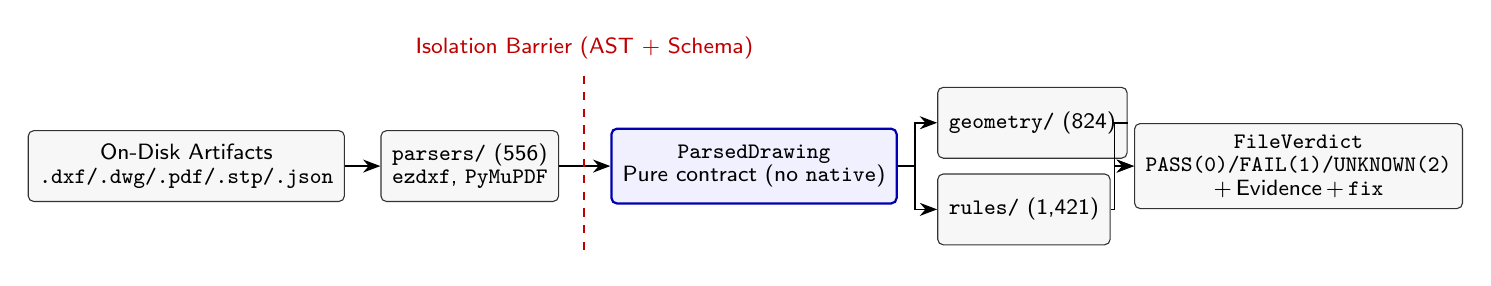
\begin{tikzpicture}[
  node distance=4.5mm and 4.5mm,
  font=\sffamily\footnotesize,
  box/.style={draw=black!80, rounded corners=2pt, fill=black!3, align=center, inner sep=4pt, minimum height=9mm},
  contract/.style={draw=blue!70!black, thick, rounded corners=2pt, fill=blue!6, align=center, inner sep=4pt, minimum height=9.5mm},
  barrier/.style={dashed, red!75!black, thick},
  arr/.style={-{Stealth[length=2.2mm]}, semithick}
]
  \node[box] (files) {On-Disk Artifacts\\[-1pt]\texttt{.dxf/.dwg/.pdf/.stp/.json}};
  \node[box, right=of files] (parsers) {\texttt{parsers/} (556)\\[-1pt]\texttt{ezdxf}, \texttt{PyMuPDF}};
  \node[contract, right=6.5mm of parsers] (pd) {\texttt{ParsedDrawing}\\[-1pt]Pure contract (no \texttt{native})};
  \node[box, right=5mm of pd, yshift=5.5mm] (geo) {\texttt{geometry/} (824)};
  \node[box, right=5mm of pd, yshift=-5.5mm] (rules) {\texttt{rules/} (1,421)};
  \node[box, right=30mm of pd] (verdict) {\texttt{FileVerdict}\\[-1pt]\texttt{PASS(0)/FAIL(1)/UNKNOWN(2)}\\[-1pt]+\,Evidence\,+\,\texttt{fix}};

  \draw[arr] (files) -- (parsers);
  \draw[arr] (parsers) -- (pd);
  \draw[arr] (pd.east) -- ++(2.2mm,0) |- (geo.west);
  \draw[arr] (pd.east) -- ++(2.2mm,0) |- (rules.west);
  \draw[arr] (geo.east) -| ([xshift=-2.5mm]verdict.west) -- (verdict.west);
  \draw[arr] (rules.east) -| ([xshift=-2.5mm]verdict.west) -- (verdict.west);

  \draw[barrier] ([xshift=3.2mm,yshift=11.5mm]parsers.east) -- ([xshift=3.2mm,yshift=-11.5mm]parsers.east);
  \node[font=\sffamily\footnotesize, text=red!75!black, align=center] at ([xshift=3.2mm,yshift=15mm]parsers.east) {Isolation Barrier (AST + Schema)};
\end{tikzpicture}%
}
\label{fig:arch_pipeline}
\end{subfigure}

\medskip
\begin{subfigure}[t]{0.98\textwidth}
\centering{
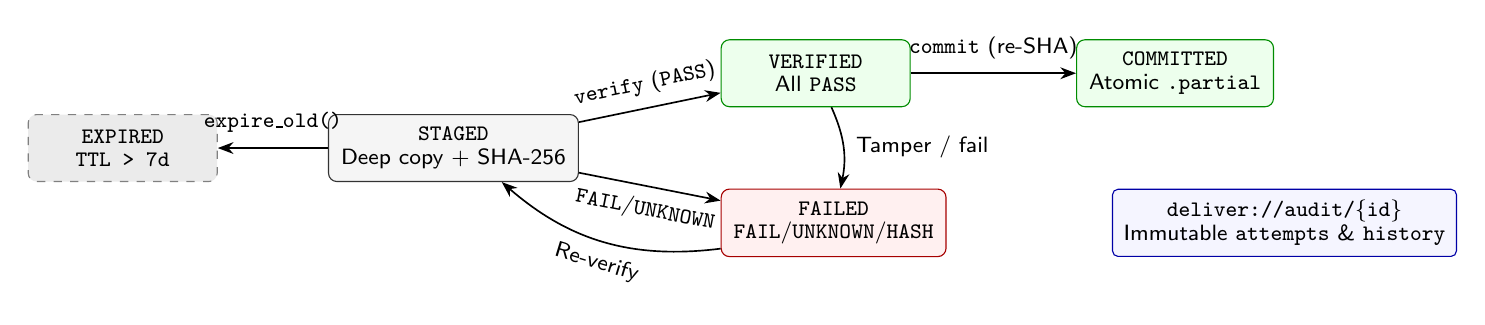
\begin{tikzpicture}[
  node distance=7.5mm and 11mm,
  font=\sffamily\footnotesize,
  st/.style={draw=black!80, rounded corners=3pt, fill=black!4, align=center, inner sep=4.5pt, minimum width=24mm, minimum height=8.5mm},
  pass/.style={st, draw=green!55!black, fill=green!7},
  fail/.style={st, draw=red!65!black, fill=red!6},
  exp/.style={st, draw=black!50, fill=black!8, dashed},
  arr/.style={-{Stealth[length=2mm]}, semithick, font=\sffamily\footnotesize}
]
  \node[st] (staged) {\texttt{STAGED}\\[-1pt]Deep copy + SHA-256};
  \node[pass, right=18mm of staged, yshift=9.5mm] (verified) {\texttt{VERIFIED}\\[-1pt]All \texttt{PASS}};
  \node[fail, right=18mm of staged, yshift=-9.5mm] (failed) {\texttt{FAILED}\\[-1pt]\texttt{FAIL}/\texttt{UNKNOWN}/\texttt{HASH}};
  \node[pass, right=21mm of verified] (committed) {\texttt{COMMITTED}\\[-1pt]Atomic \texttt{.partial}};
  \node[exp, left=14mm of staged] (expired) {\texttt{EXPIRED}\\[-1pt]\texttt{TTL > 7d}};
  \node[draw=blue!65!black, fill=blue!4, rounded corners=2pt, font=\sffamily\footnotesize, align=center, inner sep=4pt, right=21mm of failed] (audit) {\texttt{deliver://audit/\{id\}}\\[-1pt]Immutable \texttt{attempts} \& \texttt{history}};

  \draw[arr] (staged) -- node[above, sloped, yshift=1pt] {\texttt{verify} (\texttt{PASS})} (verified);
  \draw[arr] (staged) -- node[below, sloped, yshift=-1pt] {\texttt{FAIL}/\texttt{UNKNOWN}} (failed);
  \draw[arr] (verified) -- node[above, yshift=1.5pt] {\texttt{commit} (re-SHA)} (committed);
  \draw[arr] (verified) to[bend left=18] node[right, xshift=1pt] {Tamper / fail} (failed);
  \draw[arr] (failed) to[bend left=24] node[below, sloped, yshift=-1pt] {Re-verify} (staged);
  \draw[arr] (staged) -- node[above, yshift=2pt] {\texttt{expire\_old()}} (expired);
\end{tikzpicture}%
}
\label{fig:state_machine}
\end{subfigure}
\caption{System architecture and protocol semantics of \texttt{cad-deliver-mcp}: (\emph{a}) unidirectional three-layer architecture isolated by static import assertions and schema omission of live document handles; and (\emph{b}) five-state two-phase commit MCP protocol isolating staging snapshots from formal delivery directories via dual SHA-256 verification and atomic replacement\label{fig:architecture}}
\end{figure*}

\subsection{Three-State Verdict Semantics: From Silent Skips to a Three-Entry Semantic Chain}\label{sec:three_state}

Empirical evidence in Section~\ref{sec:failure_modes} showed that folding skipped checks into a pass is more hazardous than throwing a direct error, because downstream agents terminate troubleshooting and release scrap drawings as soon as they observe \texttt{PASS}. Accordingly, the gatekeeper anchors its design on a single core axiom: \textbf{\texttt{PASS} holds solely when every required dimension actually ran, its preconditions held, and no blocking violation occurred.} Three-state verdicts align across data types, severity levels, and exit codes: \texttt{Verdict.PASS} (exit code~\texttt{0}), \texttt{Verdict.FAIL} (exit code~\texttt{1}), and \texttt{Verdict.UNKNOWN} (exit code~\texttt{2}). Within the \texttt{Severity} enumeration, \texttt{BLOCKED} sits alongside \texttt{ERROR} and \texttt{WARNING} instead of under warnings, separating ``unable to execute'' from ``minor advisory.'' Table~\ref{tab:three_state_chain} summarizes the three-entry semantic chain enforcing \emph{abstention is not a pass}.

\begin{table*}[t]
\caption{Three-entry semantic chain enforcing ``abstention is not a pass'' (\texttt{UNKNOWN}, exit code 2)}\label{tab:three_state_chain}
\centering
\footnotesize
\tagpdfsetup{table/header-rows={1}}%
\begin{tabularx}{\textwidth}{L{3.1cm} L{5.4cm} L{4.2cm} Y}
\toprule
\texttt{UNKNOWN} Entry Point & Trigger Condition and Code Site & Prevented Failure Mode & Expected Caller Remediation \\
\midrule
Entry~1: Missing parser or unavailable tooling &
Absent \texttt{ezdxf}/\texttt{PyMuPDF}, corrupted file, missing DWG converter (\texttt{severity="blocked"}); unhandled rule exception caught as \texttt{E\_RULE\_CRASHED} (\texttt{Severity.BLOCKED}); upstream wrapper persists minimal \texttt{delivery.json} on core \texttt{ImportError}. &
Skipping checks when dependencies are missing yet returning \texttt{PASS}, or omitting report files so callers treat absence as ``nothing failed.'' &
Install required parser dependencies, switch to the configured virtual environment, or inspect corrupted inputs instead of treating output as pass. \\
\addlinespace[3pt]
Entry~2: Unmet rule preconditions &
\texttt{BaseStandardRule.precondition(drawing)} returns a non-empty reason; \texttt{run\_profile} emits explicit abstention record \texttt{applicable=False, code="NOT\_APPLICABLE"}. &
100\% structural false positives on mismatched artifact forms (e.g., applying single-view contour closure directly to multi-view drawings). &
Verify alignment between the exported artifact type and the selected verification profile. \\
\addlinespace[3pt]
Entry~3: Abstention on critical compliance dimensions &
\texttt{FileVerdict.verdict} inspects \texttt{CRITICAL\_RULES} (\texttt{gb.title\_block}, \texttt{gb.sheet\_size}, \texttt{gb.layer\_taxonomy}, \texttt{gb.closed\_profile}); abstention on any critical rule, or when all rules are inapplicable, forces \texttt{UNKNOWN}. (\texttt{gb.dim\_text} abstention is a semantic exemption when uniform scale is identified, not an information gap, and does not force \texttt{UNKNOWN}.) &
Accumulating 3 abstentions and 2 passes out of five enabled dimensions (four drafting-standard plus one geometric) into an overall \texttt{PASS} (e.g., SolidWorks default DXF exports). &
Supply missing layers or sheet-format entities in the source CAD exporter, or route explicitly to human drawing review. \\
\bottomrule
\end{tabularx}
\end{table*}

Under Entry~1, three-state completeness covers checker availability as well as artifact decidability. When disabling \texttt{site-packages} blocks importing the core package, the thin entry wrapper catches \texttt{ImportError}, writes a minimal \texttt{delivery.json} with \texttt{verdict: "unknown"}, \texttt{counts: \{"blocked": 1\}}, and \texttt{id: "cad\_deliver.imported"}, and exits with code~\texttt{2}. Inside \texttt{deliver\_verify}, only \texttt{Verdict.PASS} advances the staging state to \texttt{VERIFIED}; both \texttt{FAIL} and \texttt{UNKNOWN} keep the delivery gate closed (state \texttt{FAILED}) while preserving the distinct \texttt{verdict} field (with \texttt{UNKNOWN} emitting \texttt{code: "E\_NOT\_JUDGED"}), separating fixable drawing defects from insufficient information.

\subsection{Three-Way Separation of Rule Pool, Profile Manifests, and Severity Overrides}\label{sec:three_way_sep}

Conventional compliance checkers tightly couple checking logic, active rule selection, and blocking policy inside monolithic classes. Across \texttt{rules/base.py}, \texttt{rules/codes.py}, and \texttt{rules/registry.py}, we separate these concerns into three orthogonal declarative tables:

\begin{enumerate}
\item \emph{Stateless rule pool} (\texttt{\_RULES}): Every rule subclasses \texttt{BaseStandardRule} and registers via \texttt{@register\_rule}, declaring \texttt{rule\_id}, standard clause \texttt{gb\_ref}, architectural layer (\texttt{geometry} or \texttt{standard}), and default severity without binding to any profile. Its \texttt{check(drawing, ctx)} method is a pure function reporting objective facts (e.g., ``measured layout sheet size $400 \times 280$~mm'') without hardcoding blocking policy.
\item \emph{Profile enablement manifests} (\texttt{PROFILES}): A profile lists \texttt{rule\_id} keys into \texttt{\_RULES}: \texttt{LEGACY\_\allowbreak COMPAT} (empty standard rule list preserving behavioral parity with legacy \texttt{dsh-sw-cad 2.2.0}), \texttt{GEOMETRY\_\allowbreak ONLY} (generic geometric integrity only), \texttt{GB\_T\_\allowbreak TIER1} (\texttt{geo.\allowbreak bbox\_\allowbreak degenerate}, \texttt{gb.\allowbreak sheet\_\allowbreak size}, \texttt{gb.\allowbreak layer\_\allowbreak taxonomy}, \texttt{gb.\allowbreak dim\_text}, and \texttt{gb.\allowbreak title\_block}), \texttt{PROFILE\_\allowbreak CLOSURE} (isolating \texttt{gb.\allowbreak closed\_\allowbreak profile} for single-view contours), and \texttt{ISO\_216\_\allowbreak TIER1} (\texttt{gb.\allowbreak sheet\_\allowbreak size} only).
\item \emph{Machine-code severity override table} (\texttt{SEVERITY\_\allowbreak PROFILES}): \texttt{rules/\allowbreak codes.py} defines a fixed 15-code enum \texttt{Code} (9~\texttt{E\_*} errors and 6~\texttt{W\_*} warnings). Because one rule can emit findings of different gravity (e.g., \texttt{gb.\allowbreak layer\_\allowbreak taxonomy} emits blocking \texttt{E\_DIM\_\allowbreak ON\_WRONG\_\allowbreak LAYER} and non-blocking \texttt{W\_LAYER\_\allowbreak UNCLASSIFIED}), severity overrides operate on individual \texttt{Code} keys instead of whole rules.
\end{enumerate}

Code-level evidence confirms this three-way split: \texttt{gb.\allowbreak sheet\_\allowbreak size} serves both \texttt{GB\_T\_\allowbreak TIER1} and \texttt{ISO\_216\_\allowbreak TIER1} unchanged, and \texttt{E\_TITLE\_\allowbreak BLOCK} resolves to \texttt{ERROR} under \texttt{GB\_T\_\allowbreak TIER1} versus \texttt{WARNING} under \texttt{LEGACY\_\allowbreak COMPAT} without duplicating rules. Regression verification in \texttt{tests/\allowbreak golden\_\allowbreak compare.py} across 12 golden cases confirmed field-by-field parity (\texttt{PARITY OK}) between \texttt{LEGACY\_\allowbreak COMPAT} and legacy \texttt{dsh-sw-cad 2.2.0} on 2026-11-25 prior to retirement of the legacy baseline snapshot (archived in the module header of \texttt{tests/\allowbreak golden\_\allowbreak compare.py}); \texttt{tests/\allowbreak test\_\allowbreak legacy\_\allowbreak compat.py} (4~tests) further verifies non-blocking legacy compatibility, Tier-1 blocking, and exit code~\texttt{2} on corrupted inputs.

\subsection{Structured Evidence, Actionability, and Query-Level Reduction}\label{sec:actionability}

Human-facing checkers emit prose paragraphs or GUI dialogs, whereas an LLM delivery gate emits structured payloads consumed by upstream agents. We track \emph{actionability} alongside recall:
\begin{equation}\label{eqn:actionability}
\text{actionability} = \frac{\#\{\text{failing checks with an executable fix}\}}{\#\{\text{total failing checks}\}}.
\end{equation}

Every rule-layer \texttt{RuleResult} pairs six-field auditable \texttt{Evidence} (\texttt{measured}, \texttt{expected}, \texttt{location}, \texttt{handle}, \texttt{count}, \texttt{name}) with a concrete \texttt{fix} directive: \texttt{E\_PROFILE\_OPEN} reports exact millimeter coordinates of the worst dangling gap, while \texttt{E\_DIM\_TEXT\_MISMATCH} prints the offending dimension \texttt{handle} and measured value. During development, lower-level geometry and file checks in \texttt{Check} lacked \texttt{fix} guidance. Adding a \texttt{FIX\_HINTS} lookup table in \texttt{pipeline.py} across 24 core checks (e.g., instructing \texttt{\$INSUNITS = 4} for \texttt{drawing.units} and \texttt{AP214}/\texttt{AP242} export for \texttt{step.schema}, while leaving auxiliary items such as \texttt{pdf.sheet}, \texttt{pdf.text}, \texttt{review.parsed}, and \texttt{model.header} for future extension) and deduplicating blocking-first in \texttt{FileVerdict.fixes()} reaches 100\% actionability across the rule layer and 50-drawing DXF benchmark failures. Through the \texttt{L0}--\texttt{L4} lens (Section~\ref{sec:query_taxonomy}), \texttt{deliver\_verify} performs query-level reduction by running \texttt{L2} graph traversal and \texttt{L1} batch comparisons upfront so agents receive \texttt{L0} keyed coordinates and handles directly.

\subsection{Two-Phase Commit (2PC) State Machine and Atomic Delivery Protocol}\label{sec:2pc}

A stateless \texttt{verify(path)} call leaves a window between check and commit during which an agent could modify workspace files. We seal this window in \texttt{server.py} and \texttt{state\_machine.py} with a five-state two-phase commit protocol---\texttt{STAGED}, \texttt{VERIFIED}, \texttt{COMMITTED}, \texttt{FAILED}, and \texttt{EXPIRED} (Fig.~\ref{fig:state_machine})---exposed via three MCP tools and one audit resource:

\begin{enumerate}
\item \texttt{deliver\_\allowbreak stage(paths, profile=\allowbreak "GB\_T\_TIER1")} $\to$ \texttt{STAGED}: Deep-copies inputs into an isolated staging directory \texttt{\%TEMP\%/\allowbreak cad-deliver-staging/\allowbreak <16-hex UUID>/\allowbreak files/} (overridable via \texttt{CAD\_\allowbreak DELIVER\_\allowbreak STAGING}), computes byte sizes and SHA-256 digests, and writes \texttt{state.json} so later workspace edits cannot affect staged files.
\item \texttt{deliver\_verify(staging\_id)} $\to$ \texttt{VERIFIED} / \texttt{FAILED}: Increments \texttt{attempts}, appends to \texttt{history}, recomputes staged SHA-256 digests (rejecting with \texttt{E\_HASH\_CHANGED} on mismatch), and runs \texttt{pipeline.verify\_file}. Staging records older than \texttt{DEFAULT\_TTL\_DAYS = 7} days transition via \texttt{expire\_old()} to \texttt{EXPIRED} (\texttt{E\_STAGING\_EXPIRED}) while preserving history.
\item \texttt{deliver\_\allowbreak commit(staging\_id, target\_dir, overwrite=False)} $\to$ \texttt{COMMITTED}: Rejects non-\texttt{VERIFIED} records (\texttt{E\_\allowbreak NOT\_\allowbreak VERIFIED}), re-verifies SHA-256 hashes immediately before copy (\texttt{E\_\allowbreak HASH\_\allowbreak CHANGED}), and blocks filename collisions unless \texttt{overwrite=True} (\texttt{E\_\allowbreak TARGET\_\allowbreak EXISTS}), never auto-appending \texttt{\_1} or \texttt{\_v2} suffixes so version conflicts remain explicit engineering decisions.
\item \texttt{deliver://audit/\{staging\_id\}} resource: Exposes a read-only JSON log containing staged manifests, SHA-256 digests, \texttt{attempts}, full \texttt{history}, finding details, and committed paths.
\end{enumerate}

Operational robustness relies on cross-volume atomic placement (\texttt{\_atomic\_place}, writing \texttt{<name>.partial} $\to$ \texttt{os.fsync()} $\to$ \texttt{os.replace()}) and an MCP \texttt{stdio} transport guard redirecting \texttt{builtins.print} and \texttt{logging} to \texttt{stderr} before loading the MCP SDK so debug prints never corrupt JSON-RPC frames. All transitions and rejection branches pass \texttt{tests/test\_server.py} (9~tests). This 2PC layer provides auditable protocol discipline, not an adversarial security sandbox (Section~\ref{sec:protocol_boundaries}).

\subsection{Self-Review Evidence Chains, Format Boundaries, and Deployment Tensions}\label{sec:multiformat}

For SolidWorks-style self-review reports (\texttt{*\_review\_report.json}), \texttt{geometry/review\_checks.py} refuses to trust \texttt{evaluation.status == "pass"} alone. It verifies a five-fold chain: passing status, empty \texttt{review.issues}, non-empty \texttt{review.checks}, true booleans on \texttt{previews\_created}, \texttt{previews\_not\_blank}, and \texttt{expected\_outputs\_exist}, and physical existence of sibling image previews (\texttt{review.previews\_on\_disk}), emitting \texttt{review.manual} when human review is flagged. Across remaining bundle formats, Table~\ref{tab:format_capabilities} delimits exact thresholds, offline parsers, inspection depth, and \texttt{UNKNOWN} boundaries.

\begin{table*}[t]
\caption{Offline parsers, minimum byte thresholds, verification depth, and \texttt{UNKNOWN} boundaries across CAD delivery formats}\label{tab:format_capabilities}
\centering
\footnotesize
\tagpdfsetup{table/header-rows={1}}%
\begin{tabularx}{\textwidth}{L{2.9cm} r L{3.6cm} Y}
\toprule
File Format & \texttt{MIN\_BYTES} & Offline Parser & Actual Inspectable Depth and \texttt{UNKNOWN} Boundary \\
\midrule
\texttt{.dxf} & 2~KB & \texttt{ezdxf} (\texttt{parsers/dxf.py}) &
Full entity-level inspection: entities, semantic layers, \texttt{\$INSUNITS}, layouts/sheet size, scale and lineweights, CJK fonts, dimension overlap, title-block attributes, contour closure, and overridden dimension consistency; missing \texttt{ezdxf} or parse corruption emits \texttt{BLOCKED} (\texttt{UNKNOWN}). \\
\addlinespace[3pt]
\texttt{.dwg} & 2~KB & 6-byte header + converter chain (\texttt{parsers/dwg.py}) &
Validates \texttt{AC1015}--\texttt{AC1032} version headers; invokes converters in order \texttt{DSH\_SW\_CAD\_DWG\_CONVERTER} $\to$ LibreDWG \texttt{dwg2dxf} $\to$ \texttt{ODAFileConverter} into DXF before full checks; missing converter or empty output emits \texttt{drawing.entities} \texttt{BLOCKED} (\texttt{UNKNOWN}), closing the header-only pass bug. \\
\addlinespace[3pt]
\texttt{.pdf} & 1~KB & \texttt{PyMuPDF} (\texttt{parsers/pdf.py}) &
Verifies non-zero pages (\texttt{pdf.pages}), ISO~216 \texttt{A4}--\texttt{A0} ($\pm 2.0$~mm, \texttt{pdf.sheet}), and extractable vector text layer (\texttt{pdf.text}, distinguishing vector CAD plots from raster scans); missing \texttt{PyMuPDF} emits \texttt{BLOCKED} (\texttt{UNKNOWN}). \\
\addlinespace[3pt]
\texttt{.step} / \texttt{.stp} & 1~KB & Pure-text parser (\texttt{geometry/step\_checks.py}) &
Parses \texttt{FILE\_SCHEMA} (\texttt{AP203}/\texttt{AP214}/\texttt{AP242}, warning \texttt{step.pmi} on \texttt{AP203} lacking colors/assembly), counts entities ($>100$), and computes approximate 3D bounding box over raw \texttt{CARTESIAN\_POINT} coordinates (\texttt{step.bbox}, catching span $\le 10^{-6}$ degeneracy); omits $\sim 200$~MB OCCT kernel so no 3D B-rep topology reconstruction is performed. \\
\addlinespace[3pt]
Native models (\texttt{.sldprt}/\texttt{.sldasm}) & 10~KB & Binary header check (\texttt{geometry/model\_checks.py}) &
Verifies file existence, byte threshold, and SolidWorks binary signature (\texttt{model.header}), while emitting explicit \texttt{model.unchecked} warning indicating internal B-rep geometry was not inspected without a CAD runtime. \\
\bottomrule
\end{tabularx}
\end{table*}

Deploying \texttt{UNKNOWN} semantics raised three engineering trade-offs. First, leaving \texttt{dependencies} empty in \texttt{pyproject.toml} would emit \texttt{UNKNOWN} on every DXF and PDF out of the box, turning a critical diagnostic into noise; the released package pins \texttt{ezdxf>=1.3} and \texttt{pymupdf>=1.24} as mandatory defaults while isolating server transport \texttt{mcp>=1.20,<2} in an optional \texttt{[mcp]} extra for CLI users. Second, both \texttt{cad-deliver} (\texttt{cli.py}, defaulting to \texttt{LEGACY\_COMPAT} for existing \texttt{dsh-sw-cad} scripts) and \texttt{cad-deliver-mcp} (\texttt{server.py}, defaulting to \texttt{GB\_T\_TIER1} for autonomous agents) invoke the single shared kernel \texttt{pipeline.verify\_file}. Third, alongside happy-path fixtures, dedicated failure-path tests disable \texttt{site-packages} to verify exit code~\texttt{2} and minimal \texttt{delivery.json} persistence under broken environments.

%%%%%%%%%%%%%%%%%%%%%%%%%%%%%%%%%%%%%%%%%%%%%%%%%%%%%%%%%%%%%%%%%%%%%%%%%%%%%%%
\section{Domain Rule Set and Calibration}\label{sec:rules}

\subsection{Seven-Role Mechanical Drafting Layer Semantic Ontology and Cross-Standard Mapping}\label{sec:ontology}

Production engineering drawings mix Chinese and English layer names (e.g., \emph{cushixian} ``thick solid'' and \texttt{OUTLINE}), exporter plurals (\texttt{DIMENSIONS}, \texttt{CENTERLINES}), vendor prefixes (\texttt{SW-MECH-lunkuoxian}), and full-width/half-width Unicode characters, causing brittle string matching to fail whenever templates change. In \texttt{rules/taxonomy.py}, we formalize mechanical layer organization into seven semantic roles (\texttt{LayerRole}): \texttt{CONTOUR\_THICK}, \texttt{THIN\_AUX}, \texttt{CENTERLINE}, \texttt{HIDDEN\_DASHED}, \texttt{DIMENSION}, \texttt{ANNOTATION\_TEXT}, and \texttt{FRAME\_TITLE}, plus \texttt{UNCLASSIFIED} for unrecognized occupied layers while exempting built-in structural layers \texttt{STRUCTURAL\_LAYERS = \{"0", "DEFPOINTS", "DEFPOINT"\}}. Prior to matching, \texttt{normalise()} applies Unicode \texttt{NFKC} folding, underscore-to-space conversion with upper-casing, and iterative prefix stripping over \texttt{PREFIXES = ("M-", "MECH-", "SW-", "NX-", "GB-", "CAD-")}.

Supplementary Material (Table~S2) details the full bilingual alias set, priority order, entity constraints, and clause cross-walks across GB/T, ISO~128/216/7200, and ASME~Y14.1/Y14.2/Y14.5. Three roles anchor our evaluation: at priority~1, \texttt{FRAME\_\allowbreak TITLE} (\emph{tukuang}/\allowbreak\emph{biaotilan}/\allowbreak\texttt{FRAME}/\allowbreak\texttt{TITLEBLOCK}, GB/T~14689/10609.1, ISO~5457/7200, ASME~Y14.1) hosts paperspace borders and title-block inserts; at priority~2, \texttt{DIMENSION} (\emph{biaozhu}/\allowbreak\emph{chicun}/\allowbreak\texttt{DIM(S)}/\allowbreak\texttt{DIMENSION(S)}, GB/T~4458.4, ISO~129-1, ASME~Y14.5) owns all \texttt{DIMENSION}/\allowbreak\texttt{LEADER}/\allowbreak\texttt{MLEADER} entities; and at priorities~6--7, \texttt{CONTOUR\_\allowbreak THICK} (GB/T~4457.2/4457.4, ISO~128-20 Type~01, ASME~Y14.2) separates primary visible contours from \texttt{THIN\_AUX} (\emph{xishixian}, hatches, threads) via longest-alias-wins so non-contour entities stay out of closure and layer-\texttt{0} denominators.

\subsection{Deterministic Layer Disambiguation and Entity--Layer Consistency Checking}\label{sec:disambiguation}

Instead of an uninterpretable probabilistic classifier, \texttt{taxonomy.classify()} uses two deterministic rules to resolve naming collisions:

\begin{enumerate}
\item \emph{Longest-alias-wins instead of first-match-wins.} Exact normalized equality returns confidence~\texttt{1.0}. On substring fallback, matching aliases rank by descending length (returning confidence~\texttt{0.7}), resolving Chinese substring collisions such as \emph{xishixian} (``thin solid line,'' 3~characters) containing \emph{shixian} (``solid line''), and \emph{bukejian lunkuoxian} (6~characters) containing both \emph{kejian lunkuoxian} and \emph{lunkuoxian} without manual exception lists.
\item \emph{Misclassification-cost tie-breaking.} Equal-length ties resolve by engineering misclassification cost: $\texttt{FRAME\_TITLE} > \texttt{DIMENSION} > \texttt{ANNOTATION\_TEXT} > \texttt{CENTERLINE} > \texttt{HIDDEN\_DASHED} > \texttt{CONTOUR\_THICK} > \texttt{THIN\_AUX}$, setting confidence to~\texttt{0.5}, \texttt{ambiguous = True}, and \texttt{W\_LAYER\_AMBIGUOUS}. Frame errors break title blocks and dimension errors affect machining, whereas thick/thin swaps are benign.
\end{enumerate}

Unlike AutoCAD \texttt{.dws}, \texttt{gb.\allowbreak layer\_\allowbreak taxonomy} (\texttt{rules/\allowbreak gb/\allowbreak layer\_\allowbreak taxonomy.py}) inspects only occupied layers (ignoring unused preset template layers) and checks entity--layer consistency: \texttt{E\_DIM\_\allowbreak ON\_WRONG\_\allowbreak LAYER} blocks \texttt{DIMENSION}/\allowbreak\texttt{LEADER}/\allowbreak\texttt{MLEADER} entities on layer~\texttt{0} or non-\texttt{DIMENSION} roles, while \texttt{E\_CONTOUR\_\allowbreak ON\_ZERO} counts non-block modelspace contour primitives (\texttt{LINE}, \texttt{LWPOLYLINE}, \texttt{POLYLINE}, \texttt{ARC}, \texttt{CIRCLE}, \texttt{SPLINE}, \texttt{ELLIPSE}) and blocks when $\ge 50\%$ sit on layer~\texttt{0}. Early tests revealed a denominator dilution bug: counting centerlines, hatches, and borders diluted a 100\% layer-\texttt{0} contour to $2/5 = 40\%$ (silent pass). Restricting the denominator via \texttt{taxonomy.\allowbreak is\_outline\_\allowbreak layer()} to exclude the six \texttt{NON\_OUTLINE\_\allowbreak ROLES} eliminated dilution cleanly. When all occupied entities collapse onto layer~\texttt{0} or \texttt{Defpoints} (\texttt{len(occupied) == 1}), \texttt{precondition()} abstains (escalating via \texttt{CRITICAL\_\allowbreak RULES} to \texttt{UNKNOWN}), separating unlayered exporters from mislayered drafting.

\subsection{Sheet-Size and Attribute-Level Title-Block Calibration}\label{sec:sheet_title}

The sheet-size rule (\texttt{gb.sheet\_size}, GB/T~14689-2008 / ISO~216) checks layout dimensions against \texttt{A4} ($210 \times 297$~mm) through \texttt{A0} ($841 \times 1189$~mm) in portrait or landscape within \texttt{SHEET\_TOLERANCE\_MM = $\pm$2.0~mm} (tested via $\pm 1.5$~mm fixtures \texttt{gen\_11}, \texttt{gen\_12}, and \texttt{gen\_14}). Because DXF \texttt{Model} space has no paper concept yet U.S.-locale CAD setups write default \texttt{Letter} ($215.9 \times 279.4$~mm) plotter settings onto \texttt{Model}, scanning all layouts falsely rejected compliant \texttt{A3} drawings. Restricting checks and preconditions to populated non-\texttt{Model} paperspace layouts stops spurious failures and triggers abstention when paperspace is empty.

The title-block rule (\texttt{gb.title\_block}, GB/T~10609.1-2008) closes Section~\ref{sec:failure_modes}'s keyword-spoofing gap by inspecting paperspace \texttt{BlockRef} candidates identified via name tokens (\texttt{TITLE}, \emph{tukuang}, \emph{biaoti}, \texttt{FRAME}, \texttt{BORDER}, \texttt{FORMAT}, \texttt{GB-}, \texttt{GB\_}) or role \texttt{FRAME\_TITLE} across three tiers:
\begin{enumerate}
\item No candidate block reference emits blocking \texttt{E\_TITLE\_BLOCK} regardless of stray ``scale'' text (exercised by \texttt{mut\_13} and \texttt{mut\_14});
\item A candidate block lacking \texttt{ATTRIB} definitions downgrades to \texttt{W\_TITLE\_BLOCK\_NO\_ATTR} for legacy compatibility;
\item Attributed blocks must populate drawing title, drawing number, and scale in \texttt{REQUIRED\_FIELDS}, else emit \texttt{E\_TITLE\_BLOCK\_BLANK}.
\end{enumerate}
When paperspace has zero entities and zero block references, \texttt{gb.title\_block.precondition()} abstains.

\subsection{Geometric Degeneracy and Robust Contour Closure}\label{sec:bbox_profile}

The geometric degeneracy rule (\texttt{geo.bbox\_degenerate}) catches point- or line-collapsed modelspaces using \texttt{MIN\_EXTENT\_MM = 1e-3~mm} ($1~\mu$m), requiring both width and height to exceed threshold (\texttt{E\_BBOX\_DEGENERATE}) and returning silently when \texttt{extents is None}. Wiring \texttt{ezdxf.bbox.extents(msp)} in \texttt{dxf.py} fixed an early missing-extents bug. Because CAD bounds traverse circle radii, text heights, and cached \texttt{*D} blocks on \texttt{DIMENSION} entities, all three spans govern the mutation-purity operator in Section~\ref{sec:benchmark_design}.

Contour closure analysis (\texttt{geometry/\allowbreak topology.py} and \texttt{gb.\allowbreak closed\_\allowbreak profile}) avoids commercial-export false positives from \texttt{entity.closed = False} flags through three constraints: (1) classifying polylines as closed when \texttt{bool(entity.closed) or \_close(p0, p[-1], 0.01~mm)} holds (\texttt{gen\_02}, \texttt{05}, \texttt{08}, \texttt{12}, \texttt{13}, \texttt{15}); (2) building a Union-Find graph over open primitives under \texttt{JOIN\_\allowbreak TOLERANCE\_MM = 0.01~mm} and reporting \texttt{degree == 1} gap coordinates; and (3) filtering out \texttt{CIRCLE}, non-boundary types (\texttt{POINT}, \texttt{SOLID}, \texttt{HATCH}, \texttt{DIMENSION}), and \texttt{is\_outline\_\allowbreak layer()}-excluded roles. Implementing 0.01~mm snapping exposed an instructive quantization-grid half-cell trap: naive \texttt{round(x / 0.01)} strands 0.008~mm export noise across cell boundaries. Querying a 9-cell neighborhood spatial hash \texttt{\_VertexIndex} with Chebyshev distance ($|\Delta x|, |\Delta y| \le 0.01$~mm) enforces the specification (locked by 13 tests in \texttt{tests/\allowbreak test\_\allowbreak topology.py}). Because multi-view orthographic drawings legitimately contain open edges, \texttt{gb.\allowbreak closed\_\allowbreak profile} lives in isolated \texttt{PROFILE\_\allowbreak CLOSURE}.

\subsection{Dimension-Text Consistency: Separating Systematic Scaling From Isolated Errors}\label{sec:dim_text}

Overwriting dimension text to contradict geometry creates severe manufacturing risk because machinists cut to printed numerals. Rule \texttt{gb.dim\_text} (GB/T~4458.4-2003) checks overridden linear modelspace dimensions (skipping \texttt{""}, \texttt{"<>"}, scaled \texttt{dimlfac != 1.0}, and angular/ordinate \texttt{dimtype in (2, 5, 6)}) under $\max(0.01\text{~mm}, 0.2\% \times |\text{expected}|)$. To distinguish scaled views (e.g., $1{:}2$) from tampered numerals without trusting title-block text, we compute $r_i = \text{shown}_i / \text{expected}_i$, sample mean $\bar{r}$, and $\text{spread} = \max_i |r_i - \bar{r}| / |\bar{r}|$ in \texttt{rules/gb/dim\_text.py}:

\begin{itemize}
\item When mismatched count exceeds~1, $\text{spread} < 0.01$, and $|\bar{r} - 1.0| > 0.01$, all mismatches reflect a shared scale multiplier; the rule infers a scaled view and abstains (\texttt{ok = True, applicable = False}).
\item When only one dimension mismatches, the rule exempts it only if $r_1$ lies within $\pm 1\%$ of $\{0.1, 0.2, 0.25, 0.5,\allowbreak 2.0, 4.0, 5.0, 10.0\}$, otherwise emitting \texttt{E\_DIM\_\allowbreak TEXT\_\allowbreak MISMATCH} (\texttt{FAIL}).
\end{itemize}

Real SolidWorks~2025 exports confirm this separation: \texttt{part-012} carries 8 dimensions all at $21.0/3.000 = 7.0000\times$ ($\text{spread}=0$) and is exempted as scaled, whereas \texttt{part-013} carries one mismatch at $8.0/6.000 = 1.3333\times$ and triggers \texttt{FAIL}. Beyond CAD, ratio-dispersion gating separates systematic unit errors ($\times 25.4$, $\times 1000$) from point tampering. Note that \texttt{gb.dim\_text} abstention is a \emph{semantic exemption} based on positively identifying a scale factor, not an information gap, so it is deliberately excluded from \texttt{CRITICAL\_RULES}. Supplementary Material (Table~S3) consolidates parameters for all six rules.

\subsection{Domain Artifact Boundary: Engineering-Drawing DXF Versus Model-Export DXF}\label{sec:dxf_modes}

Commercial DXF export is not configuration-invariant: exporting \texttt{PART-001.sldprt} from SolidWorks~2025 under three settings yielded three incompatible DXF forms. Default \texttt{SaveAs} $\to$ \texttt{DXF} emitted 13 modelspace entities (9~\texttt{LINE} + 4~\texttt{LWPOLYLINE}), 0 paperspace entities, \texttt{\$INSUNITS = 1} (inches), all geometry on layer~\texttt{0}, 0 dimensions, and empty \texttt{Layout1}/\texttt{Layout2}. Enabling \texttt{swDxfAllSheetsToPaperSpace = on} wrote \texttt{0} modelspace entities, 21 paperspace entities, and \texttt{\$INSUNITS = 4} (millimeters), immediately tripping \texttt{drawing.entities} zero-entity failures without adding any real sheet format. Disabling that flag while inserting standard 3-views and model dimensions produced 20 modelspace entities (18~\texttt{LINE} + 2~\texttt{DIMENSION}), 0 paperspace entities, and \texttt{\$INSUNITS = 4}, still omitting borders, title block, and semantic layers.

This probe yields three methodological and engineering lessons: API flags such as \texttt{swDxfAllSheetsToPaperSpace} can relocate geometry into paperspace without writing sheet metadata; ``engineering-drawing DXF'' must be separated from flat ``model-export DXF'' (implemented in \texttt{benchmarks/run\_eval.py} via \texttt{looks\_like\_engineering\_drawing()}); and commercial export benchmarks must preserve zero post-processing and exact export settings, justifying our split between AutoCAD \texttt{fixtures/real/} and SolidWorks \texttt{fixtures/real\_sw/} in Section~\ref{sec:eval}.

%%%%%%%%%%%%%%%%%%%%%%%%%%%%%%%%%%%%%%%%%%%%%%%%%%%%%%%%%%%%%%%%%%%%%%%%%%%%%%%
\section{Experimental Evaluation}\label{sec:eval}

\subsection{Fifty-Drawing Hybrid Benchmark Construction and the Mutation-Purity Criterion}\label{sec:benchmark_design}

To test whether the gatekeeper separates deliverable engineering drawings from syntactically openable defective artifacts, we constructed a 50-drawing hybrid benchmark (\texttt{benchmarks/tasks.json} and \texttt{benchmarks/mutations.json}) plus a 15-part cross-ecosystem suite:

\begin{itemize}
\item \emph{Compliant suite ($n = 30$).} Half (\texttt{fixtures/real/}, $n = 15$) comprises native \texttt{Document.Export} DXFs from AutoCAD~2025 (\texttt{PART-001}--\texttt{PART-015}) spanning three sheets ($\texttt{A4} \times 5$, $\texttt{A3} \times 7$, $\texttt{A2} \times 3$), three scales ($1{:}1$, $1{:}2$, $2{:}1$), and 15 parts under zero post-processing. The other half (\texttt{fixtures/gen/}, $n = 15$) comprises \texttt{ezdxf}-generated drawings (\texttt{gen\_01}--\texttt{gen\_15}) covering \texttt{A0}--\texttt{A4} portrait and landscape layouts, $\pm 1.5$~mm tolerance boundaries (within $\pm 2.0$~mm), and \texttt{closed = False} closed contours, self-verified against \texttt{GB\_T\_TIER1} at generation.
\item \emph{Defect-injection suite ($n = 20$).} Built by \texttt{benchmarks/mutate.py} via alternating draws across 10 AutoCAD (\texttt{PART-001}--\texttt{PART-010}) and 10 generated (\texttt{gen\_01}--\texttt{gen\_10}) drawings, each sample carries one targeted defect across 6 categories and 7 error codes: \texttt{E\_BBOX\_DEGENERATE} (4), \texttt{E\_PROFILE\_OPEN} (4, under \texttt{PROFILE\_CLOSURE}), \texttt{E\_SHEET\_SIZE} (4, set to $400 \times 280$~mm), \texttt{E\_TITLE\_BLOCK} (2, block deleted while retaining paperspace ``scale'' text), \texttt{E\_TITLE\_BLOCK\_BLANK} (2, mandatory attributes cleared), \texttt{E\_DIM\_ON\_WRONG\_LAYER} (2, dims moved to contour layer), and \texttt{E\_CONTOUR\_ON\_ZERO} (2, contours moved to layer~\texttt{0}). Manifest generation aborts on any mismatch.
\item \emph{Cross-ecosystem suite ($n = 15$).} \texttt{fixtures/real\_sw/} holds native SolidWorks~2025 \texttt{SaveAs} $\to$ \texttt{DXF} exports of the identical 15 parts (\texttt{part-001}--\texttt{part-015}). Because default exports omit layers and sheet formats and trigger \texttt{UNKNOWN}, these files stay separate from the 30-compliant FP denominator.
\end{itemize}

Constructing \texttt{mut\_01}--\texttt{mut\_04} revealed a methodological requirement for clean ablation attribution, \emph{mutation purity}: an injected mutation may only alter semantics isomorphic to the target rule while preserving all non-target semantics. Deleting modelspace entities let \texttt{LEGACY\_COMPAT} claim a confounded 4/20 recall via its pre-existing zero-entity check (\texttt{drawing.entities}). Our corrected \texttt{collapse\_bbox} operator keeps all entities while flattening coordinates onto $(0,0)$, requiring \texttt{\_flatten()} to collapse three implicit spans simultaneously: setting \texttt{CIRCLE}/\texttt{ARC} radii to $10^{-9}$, setting \texttt{TEXT}/\texttt{MTEXT}/\texttt{ATTRIB} heights to $10^{-9}$ (removing 3.5~mm text boxes), and stripping \texttt{*D} anonymous-block \texttt{geometry} references on \texttt{DIMENSION} entities. Under pure mutations, \texttt{LEGACY\_COMPAT} drops to 0/20 recall, isolating all 4/4 detections to \texttt{geo.bbox\_degenerate}.

\subsection{Main Benchmark Five-Arm Comparison, Clopper--Pearson Bounds, and Latency Overhead}\label{sec:main_results}

On the 50-drawing main benchmark (\texttt{benchmarks/run\_eval.py}), we compare five cumulative gating arms: \texttt{G1} (no gate, unconditional \texttt{PASS}), \texttt{G2} (file exists and non-empty bytes), \texttt{G2.5} (static-syntax script: openable by \texttt{ezdxf}, non-empty modelspace entities, and \texttt{\$INSUNITS != 0}), \texttt{LEGACY\_COMPAT} (legacy \texttt{dsh-sw-cad 2.2.0}), and \texttt{G3} (full gatekeeper: \texttt{GB\_T\_TIER1} plus sample-routed \texttt{PROFILE\_CLOSURE}). Table~\ref{tab:main_benchmark} compiles all five arms alongside AutoCAD \texttt{.dws} and \texttt{qwen3-vl-plus}:

\begin{enumerate}
\item \emph{Blindness of static-syntax baselines.} \texttt{G1}, \texttt{G2}, \texttt{G2.5}, and \texttt{LEGACY\_COMPAT} all score 0/20 total recall (0/4 geometry and 0/16 standards): openable DXFs with entities and non-zero units still fail compliance rules.
\item \emph{Clopper--Pearson statistical bounds.} Full gatekeeper \texttt{G3} achieves 20/20 (100.0\%) exact machine-code recall alongside 0/30 (0.0\%) compliant false positives. Exact one-sided 95\% binomial intervals (\texttt{math.comb}) yield an 86.1\% recall lower bound ($0.05^{1/20}$) and a 9.5\% FP upper bound ($1 - 0.05^{1/30}$). Because subclasses have $n \le 4$ (95\% lower bound 47.3\% at $n = 4$), Panel~B per-class counts are descriptive only.
\item \emph{Millisecond rule overhead.} Across all 50 drawings, the frozen latency snapshot (\texttt{benchmarks/\allowbreak results/\allowbreak latency.csv}) records \texttt{G3} median latency $p_{50} = 12.37$~ms ($p_{95} = 50.75$~ms) versus \texttt{G2.5} at $10.30$~ms ($p_{95} = 43.88$~ms), placing net median overhead of the six rules at 2.07~ms (tail variance reflects parsing/classification without per-file frozen breakdowns; Table~\ref{tab:main_benchmark} notes record the consistent pre-freeze main run at \texttt{G3} 12.65/51.98~ms, net 2.46~ms).
\end{enumerate}

\begin{table*}[t]
\caption{Main 50-drawing benchmark comparison across five gating arms, commercial \texttt{.dws}, and VLM visual review, with descriptive per-defect breakdown}\label{tab:main_benchmark}
\centering
\scriptsize
\setlength{\tabcolsep}{2.5pt}
\begin{minipage}{\textwidth}
\tagpdfsetup{table/header-rows={1}}%
\begin{tabularx}{\textwidth}{Y c r c r r c r r}
\multicolumn{9}{l}{\textbf{Panel A: Overall defect recall, exact attribution, compliant false positives, and latency ($n=50$: 30 compliant = 15 AutoCAD + 15 generated; 20 injected defects)}} \\
\toprule
Baseline / Gating Arm & Recall ($n=20$) & CP 95\% LB & Exact Code / Rationale ($n=20$) & Compliant FP ($n=30$) & CP 95\% UB & Machine Verdict & $p_{50}$ (ms) & $p_{95}$ (ms) \\
\midrule
\texttt{G1} (No gate / always \texttt{PASS}) & 0/20 (0.0\%) & 0.0\% & 0/20 & 0/30 (0.0\%) & 9.5\% & Yes & 0.002 & 0.002 \\
\texttt{G2} (File exists \& non-empty) & 0/20 (0.0\%) & 0.0\% & 0/20 & 0/30 (0.0\%) & 9.5\% & Yes & 0.194 & 0.340 \\
\texttt{G2.5} (Syntax: \texttt{ezdxf} + entities + units) & 0/20 (0.0\%) & 0.0\% & 0/20 & 0/30 (0.0\%) & 9.5\% & Yes & 10.30 & 43.88 \\
\texttt{LEGACY\_COMPAT} (\texttt{dsh-sw-cad 2.2.0}) & 0/20 (0.0\%) & 0.0\% & 0/20 & 0/30 (0.0\%) & 9.5\% & Yes & 11.55 & 33.37 \\
AutoCAD \texttt{.dws} (30-compliant union) & 0/20 (0.0\%) & 0.0\% & 0/20 & ---$^{a}$ & --- & \textbf{No} (GUI modal) & N/A & N/A \\
VLM (\texttt{qwen3-vl-plus}, 150-DPI PNG) & 19/20 (95.0\% ref.) & ---$^{b}$ & \textbf{11/20 (55.0\%)} & \textbf{17/30 (56.7\%)}$^{c}$ & --- & \textbf{No} (prose JSON) & --- & --- \\
\textbf{\texttt{G3} (\texttt{cad-deliver-mcp} full gate)} & \textbf{20/20 (100.0\%)} & \textbf{86.1\%} & \textbf{20/20 (100.0\%)} & \textbf{0/30 (0.0\%)} & \textbf{9.5\%} & \textbf{Yes} (code+evid.+fix) & \textbf{12.37} & \textbf{50.75} \\
\bottomrule
\end{tabularx}

\vspace{6pt}
\begin{tabularx}{\textwidth}{Y c l r r r r r c r}
\multicolumn{10}{l}{\textbf{Panel B: Descriptive detection breakdown across 6 report categories expanded into 7 machine error codes ($n=20$; title block split by missing block vs.\ blank attribute)}} \\
\toprule
Defect Category \& Machine Code & Layer & Modality & $n$ & \texttt{G2.5} & \texttt{LEGACY} & \texttt{.dws} & VLM Refusal & VLM Rationale & \texttt{G3} Exact \\
\midrule
Bbox degeneracy (\texttt{E\_BBOX\_DEGENERATE}) & \texttt{geometry} & Visual/Geom. & 4 & 0/4 & 0/4 & 0/4 & 4/4 & \textbf{4/4} & \textbf{4/4} \\
Open contour (\texttt{E\_PROFILE\_OPEN})$^{d}$ & \texttt{standard} & Visual/Geom. & 4 & 0/4 & 0/4 & 0/4 & 4/4 & \textbf{3/4} (miss \texttt{mut\_07}) & \textbf{4/4} \\
Missing title block (\texttt{E\_TITLE\_BLOCK}) & \texttt{standard} & Visual/Geom. & 2 & 0/2 & 0/2 & 0/2 & 2/2 & \textbf{2/2} & \textbf{2/2} \\
Blank title attr.\ (\texttt{E\_TITLE\_BLOCK\_BLANK}) & \texttt{standard} & Visual/Geom. & 2 & 0/2 & 0/2 & 0/2 & 2/2 & \textbf{2/2} & \textbf{2/2} \\
\emph{Subtotal: Visual / Geometric} & --- & --- & \textbf{12} & 0/12 & 0/12 & 0/12 & 12/12 & \textbf{11/12 (91.7\%)} & \textbf{12/12} \\
Non-standard sheet (\texttt{E\_SHEET\_SIZE}, $400{\times}280$) & \texttt{standard} & Meta./Attr. & 4 & 0/4 & 0/4 & 0/4 & 3/4 (pass \texttt{mut\_10}) & \textbf{0/4} & \textbf{4/4} \\
Mislayered dims (\texttt{E\_DIM\_ON\_WRONG\_LAYER}) & \texttt{standard} & Meta./Attr. & 2 & 0/2 & 0/2 & 0/2 & 2/2 & \textbf{0/2} & \textbf{2/2} \\
Contour on layer~0 (\texttt{E\_CONTOUR\_ON\_ZERO}) & \texttt{standard} & Meta./Attr. & 2 & 0/2 & 0/2 & 0/2 & 2/2 & \textbf{0/2} & \textbf{2/2} \\
\emph{Subtotal: Layer / Sheet Metadata} & --- & --- & \textbf{8} & 0/8 & 0/8 & 0/8 & 7/8 & \textbf{0/8 (0.0\%)} & \textbf{8/8} \\
\textbf{Total (\texttt{ALL})} & \texttt{both} & \texttt{both} & \textbf{20} & \textbf{0/20} & \textbf{0/20} & \textbf{0/20} & \textbf{19/20 (95.0\%)} & \textbf{11/20 (55.0\%)} & \textbf{20/20 (100.0\%)} \\
\bottomrule
\end{tabularx}
\par\smallskip\footnotesize
Notes: $^{a}$The \texttt{.dws} reference merges the four named tables across all 30 compliant drawings (using only the 15 AutoCAD drawings triggers 10/20 cross-generator false positives from \texttt{ezdxf} styles; see Section~\ref{sec:dws}); compliant FP and upper bound are marked ``---'' because passing the union of itself holds by definition and only 0/20 defect recall is evaluated. $^{b}$VLM 19/20 (95.0\%) reflects high-false-positive binary refusal instead of true defect localization. $^{c}$VLM 17/30 (56.7\%) false positives comprise 14/15 AutoCAD drawings (only \texttt{PART-004} passed) and 3/15 generated drawings (\texttt{gen\_08}, \texttt{gen\_09}, \texttt{gen\_10}), partly influenced by \texttt{TextPolicy.IGNORE} hiding dimension numerals (Section~\ref{sec:render_debug}). $^{d}$\texttt{E\_PROFILE\_OPEN} is evaluated under \texttt{PROFILE\_CLOSURE}; Panel~B subclasses ($n \le 4$; 95\% CP LB 47.3\% at $n=4$) are descriptive only. Latency numbers report the frozen repository snapshot \texttt{benchmarks/results/latency.csv} (commit \texttt{9bb9d1d}: \texttt{G3} $p_{50}=12.37$~ms / $p_{95}=50.75$~ms; net rule overhead 2.07~ms); the prior pre-freeze main run recorded \texttt{G1} 0.002/0.002, \texttt{G2} 0.197/0.370, \texttt{G2.5} 10.19/47.25, \texttt{LEGACY\_COMPAT} 11.78/34.34, and \texttt{G3} 12.65/51.98~ms (net 2.46~ms), consistent within the same millisecond regime.
\end{minipage}
\end{table*}

\subsection{Leave-One-Out (LOO) Rule Ablation Study}\label{sec:loo}

To test rule non-redundancy, we ran a leave-one-out ablation across all 50 benchmark tasks (\texttt{benchmarks/results/ablation\_loo.csv}), removing one rule at a time from \texttt{GB\_T\_TIER1} + \texttt{PROFILE\_CLOSURE} (full baseline: 20/20 recall, 1.0000 rate, 0/30 FP). Removing any of five rules drops recall by exactly $-4$ to 16/20 (0.8000) while keeping 0/30 compliant FP (0 FP delta), confirming mutual orthogonality with zero inter-rule masking: \texttt{geo.bbox\_degenerate} solely catches \texttt{mut\_01}--\texttt{mut\_04}; \texttt{gb.sheet\_size} catches \texttt{mut\_09}--\texttt{mut\_12}; \texttt{gb.layer\_taxonomy} catches \texttt{mut\_17}--\texttt{mut\_18} (dim layer) and \texttt{mut\_19}--\texttt{mut\_20} (layer~\texttt{0}); \texttt{gb.title\_block} catches \texttt{mut\_13}--\texttt{mut\_14} (no block) and \texttt{mut\_15}--\texttt{mut\_16} (blank attributes); and \texttt{gb.closed\_profile} catches \texttt{mut\_05}--\texttt{mut\_08}.

By contrast, removing \texttt{gb.dim\_text} produces a 0 recall drop (20/20, 0/30 FP). We report this transparently: our 20 synthetic defects span 6 categories without an overridden dimension-text mutation, so the 0 drop reflects synthetic benchmark coverage, not redundancy. Outside the synthetic split, \texttt{gb.dim\_text} is the sole rule separating uniform scaling (\texttt{part-012}, 8 dims at $7.0000\times$) from isolated mismatch (\texttt{part-013}, $1.3333\times$) in SolidWorks~2025 exports, and catches $+0.3\%$ text overrides in \texttt{complex\_03\_dim\_text} and \texttt{complex\_06\_all\_four} (Section~\ref{sec:discussion}).

\subsection{Commercial Built-In Baseline: AutoCAD CAD Standards (\texttt{.dws})}\label{sec:dws}

To test whether commercial built-in checkers can serve as an automated delivery gate, we ran AutoCAD~2025 COM probes alongside \texttt{scripts/\allowbreak eval\_\allowbreak autocad\_\allowbreak dws.py} (\texttt{benchmarks/\allowbreak results/\allowbreak baseline\_\allowbreak dws.csv}). On automation integrability, headless \texttt{.dws} execution failed on AutoCAD~2025: \texttt{AcadDocument.SaveAs} rejected all attempted format constants (\texttt{0, 1, 2, 3, 4, 5, 6, 8}), and \texttt{\_-\allowbreak CHECKSTANDARDS} ran strictly as an interactive modal dialog without writing a report or exposing any member on late-bound \texttt{AcadDocument} (\texttt{emits\_\allowbreak machine\_\allowbreak verdict = no}).

On theoretical detection capability, a \texttt{.dws} file inspects four named tables (\texttt{layers}, \texttt{linetypes}, \texttt{text\_styles}, \texttt{dim\_styles}). Merging those tables across all 30 compliant drawings (excluding built-in AutoCAD entries \texttt{Defpoints}, \texttt{Annotative}, \texttt{\_ARCHTICK}, \texttt{\_CLOSED}, and \texttt{\$}) yielded 0/20 recall on the 20 defective files: none of the six injected defects creates an illicit named table entry. Building this baseline also revealed a cross-generator default-style trap: building the \texttt{.dws} union solely from the 15 native AutoCAD files (\texttt{fixtures/real/}) flagged 10/20 defects purely because \texttt{ezdxf} defaults (\emph{xishixian}, \texttt{CENTER2}, \texttt{LiberationMono}, \texttt{EZDXF}) differed from AutoCAD templates; expanding the reference to all 30 compliant drawings removed that artifact.

\subsection{VLM Visual Baseline: Apparent Refusal Versus Rationale-Matched Recall}\label{sec:vlm_gap}

To evaluate visual review by VLMs, \texttt{scripts/render\_dxf\_png.py} rendered all 65 DXFs (15 AutoCAD, 15 generated compliant, 20 mutated, 15 SolidWorks) as 150-DPI color PNGs (white background, layer colors preserved, $1.4\times$ lineweight scaling, sheet border drawn). We then ran \texttt{qwen3-vl-plus} (\texttt{benchmarks/eval\_vlm.py}) with a uniform five-question JSON prompt (\texttt{sheet\_ok}, \texttt{layers\_ok}, \texttt{title\_block\_ok}, \texttt{closed\_ok}, \texttt{dims\_ok}) plus a \texttt{finding} summary and confidence tag (\texttt{benchmarks/results/baseline\_vlm.csv}, \texttt{baseline\_vlm\_scored.csv}, \texttt{baseline\_vlm.md}).

Results diverge sharply between apparent rejection and genuine defect matching (Table~\ref{tab:main_benchmark} Panel~A and Fig.~\ref{fig:vlm_metric_gap}):
\begin{itemize}
\item Apparent binary refusal rate on defects: 19/20 (95.0\%), with only \texttt{mut\_10\_sheet\_size} passing at high confidence.
\item Rationale-matched defect recall: 11/20 (55.0\%).
\item Compliant false-positive rate: 17/30 (56.7\%), covering 14/15 AutoCAD drawings (only \texttt{PART-004} passed) and 3/15 generated drawings (\texttt{gen\_08\_a1\_landscape}, \texttt{gen\_09\_a0\_portrait}, \texttt{gen\_10\_a0\_landscape}); all 15/15 SolidWorks comparison files were rejected with \texttt{low} confidence.
\end{itemize}

Apparent refusal (95.0\%) nearly doubles true localization recall (55.0\%) because a classifier rejecting almost every image scores high apparent recall; refusal rate alone therefore measures threshold calibration, not verification capability. In \texttt{benchmarks/score\_vlm.py}, every defective case records binary verdict and verbatim model rationales (\texttt{basis} in \texttt{baseline\_vlm\_scored.csv}). On identical inputs, deterministic rules outperform \texttt{qwen3-vl-plus} in both accuracy (20/20 exact codes, 0/30 FP vs.\ 11/20 rationale-matched, 17/30 FP) and utility (handles, coordinates, and repair instructions vs.\ 9/20 prose responses blaming unrelated artifacts).

\begin{figure*}[t]
\begin{subfigure}[t]{0.38\textwidth}
\centering{
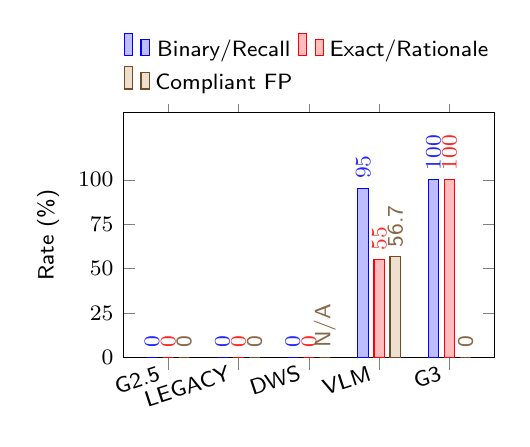
\begin{tikzpicture}
\begin{axis}[
  ybar=2pt,
  width=6.3cm, height=4.7cm,
  bar width=3.8pt,
  ymin=0, ymax=138,
  ylabel={Rate (\%)},
  label style={font=\sffamily\footnotesize},
  tick label style={font=\sffamily\footnotesize},
  symbolic x coords={G2.5, LEGACY, DWS, VLM, G3},
  xtick=data,
  x tick label style={font=\sffamily\footnotesize, rotate=18, anchor=east},
  enlarge x limits=0.16,
  ytick={0,25,50,75,100},
  legend style={at={(0.5,1.03)}, anchor=south, legend columns=2, font=\sffamily\footnotesize, draw=none},
  nodes near coords,
  nodes near coords style={font=\sffamily\footnotesize, rotate=90, anchor=west},
  every axis plot/.append style={fill opacity=0.85}
]
\addplot coordinates {(G2.5,0) (LEGACY,0) (DWS,0) (VLM,95.0) (G3,100.0)};
\addplot coordinates {(G2.5,0) (LEGACY,0) (DWS,0) (VLM,55.0) (G3,100.0)};
\addplot+[point meta=explicit symbolic] coordinates {(G2.5,0) [0] (LEGACY,0) [0] (DWS,0) [N/A] (VLM,56.7) [56.7] (G3,0) [0]};
\legend{Binary/Recall, Exact/Rationale, Compliant FP}
\end{axis}
\end{tikzpicture}%
\label{fig:vlm_metric_gap}
}%
\end{subfigure}%
\hfill
\begin{subfigure}[t]{0.30\textwidth}
\centering{
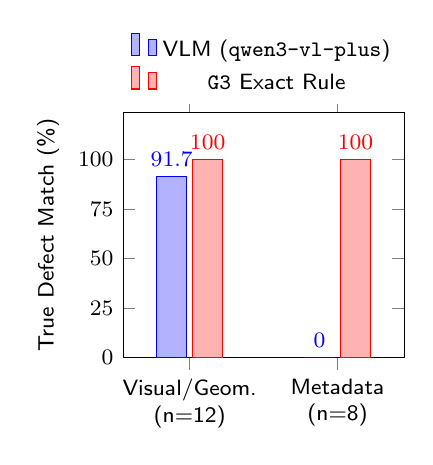
\begin{tikzpicture}
\begin{axis}[
  ybar,
  width=5.15cm, height=4.7cm,
  bar width=11pt,
  ymin=0, ymax=124,
  ylabel={True Defect Match (\%)},
  label style={font=\sffamily\footnotesize},
  tick label style={font=\sffamily\footnotesize},
  symbolic x coords={vg, meta},
  xtick=data,
  xticklabels={Visual/Geom.\\(n=12), Metadata\\(n=8)},
  x tick label style={font=\sffamily\footnotesize, align=center},
  enlarge x limits=0.45,
  ytick={0,25,50,75,100},
  legend style={at={(0.5,1.03)}, anchor=south, legend columns=1, font=\sffamily\footnotesize, draw=none},
  nodes near coords,
  nodes near coords style={font=\sffamily\footnotesize}
]
\addplot coordinates {(vg, 91.7) (meta, 0.0)};
\addplot coordinates {(vg, 100.0) (meta, 100.0)};
\legend{VLM (\texttt{qwen3-vl-plus}), \texttt{G3} Exact Rule}
\end{axis}
\end{tikzpicture}%
\label{fig:vlm_modality_split}
}%
\end{subfigure}%
\hfill
\begin{subfigure}[t]{0.30\textwidth}
\centering{
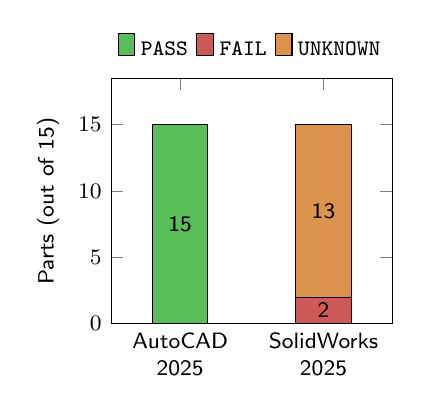
\begin{tikzpicture}
\begin{axis}[
  ybar stacked,
  width=5.15cm, height=4.7cm,
  bar width=20pt,
  ymin=0, ymax=18.5,
  ylabel={Parts (out of 15)},
  label style={font=\sffamily\footnotesize},
  tick label style={font=\sffamily\footnotesize},
  symbolic x coords={acad, sw},
  xtick=data,
  xticklabels={AutoCAD\\2025, SolidWorks\\2025},
  x tick label style={font=\sffamily\footnotesize, align=center},
  enlarge x limits=0.48,
  ytick={0,5,10,15},
  legend style={at={(0.5,1.03)}, anchor=south, legend columns=3, font=\sffamily\footnotesize, draw=none, /tikz/every even column/.append style={column sep=1pt}},
  nodes near coords,
  point meta=explicit symbolic,
  nodes near coords style={font=\sffamily\footnotesize, text=black}
]
\addplot[fill=green!60!black!65] coordinates {(acad, 15) [15] (sw, 0) []};
\addplot[fill=red!70!black!65] coordinates {(acad, 0) [] (sw, 2) [2]};
\addplot[fill=orange!80!black!70] coordinates {(acad, 0) [] (sw, 13) [13]};
\legend{\texttt{PASS}, \texttt{FAIL}, \texttt{UNKNOWN}}
\end{axis}
\end{tikzpicture}%
\label{fig:cross_ecosystem}
}%
\end{subfigure}%
\caption{Quantitative benchmark and cross-ecosystem comparisons: (\emph{a}) 50-drawing baseline gap separating VLM binary refusal (95.0\%) from rationale-matched recall (55.0\%) and compliant false positives (56.7\%); (\emph{b}) VLM capability cliff between visual/geometric (91.7\%) and metadata (0.0\%) defects versus \texttt{G3} (100.0\%); and (\emph{c}) cross-ecosystem verdicts under identical \texttt{GB\_T\_TIER1} rules on 15 identical mechanical parts (note: \texttt{.dws} compliant FP marked N/A reflects its 30-compliant union definition per Table~\ref{tab:main_benchmark} note~a)\label{fig:benchmark_charts}}
\end{figure*}

\subsection{VLM Capability Split: Visual/Geometric (11/12) Versus Metadata (0/8) and Pixel Proof}\label{sec:vlm_split}

Breaking down \texttt{qwen3-vl-plus} rationale-matched detections by modality (Table~\ref{tab:main_benchmark} Panel~B and Fig.~\ref{fig:vlm_modality_split}) exposes a steep cliff between visual image facts and symbolic metadata:

\begin{itemize}
\item \emph{Visual and geometric defects (12 cases, 11/12 = 91.7\% rationale match).} \texttt{E\_BBOX\_DEGENERATE} hits 4/4 (citing blank sheets or \texttt{"one red dot --- no geometry"}); \texttt{E\_PROFILE\_OPEN} hits 3/4 (spotting gaps in \texttt{mut\_05}/\texttt{06}/\texttt{08} while claiming \texttt{"outline is closed"} on \texttt{mut\_07\_profile\_open}); and \texttt{E\_TITLE\_BLOCK} and \texttt{E\_TITLE\_BLOCK\_BLANK} hit 2/2 and 2/2.
\item \emph{Layer and sheet metadata defects (8 cases, 0/8 = 0.0\% rationale match).} \texttt{E\_SHEET\_SIZE} ($400 \times 280$~mm) hits 0/4 (misread as valid \texttt{A3} or passed in \texttt{mut\_10}, with the rest rejected on unrelated title-block guesses); \texttt{E\_DIM\_ON\_WRONG\_LAYER} hits 0/2 (layers unmentioned); and \texttt{E\_CONTOUR\_ON\_ZERO} hits 0/2 (blamed on cropping/monochrome rendering).
\end{itemize}

This 11/12 versus 0/8 boundary reflects physical encoding, not prompting. On \texttt{E\_CONTOUR\_ON\_ZERO}, layer~\texttt{0} and the contour layer both plot in ACI color~7. Direct RGB histograms on the evaluated PNGs verify that defective \texttt{mut\_19\_contour\_on\_zero.png} has 1,098 non-white chromatic pixels out of 18,919 non-white pixels (5.8\%) versus 1,150 out of 22,159 (5.2\%) in compliant \texttt{PART-002.png} (where chromatic denotes non-gray pixels at chroma threshold $\max(R,G,B) - \min(R,G,B) > 30/255$); in both images, 100\% of chromatic pixels belong to the red ACI-1 centerline crosshairs (including anti-aliased centerline--contour intersections), leaving 0 chromatic pixels on the contour itself. The VLM's remark on \texttt{mut\_19}---\texttt{"No line colours are visible (monochrome)"}---correctly describes the bitmap yet misassigns the cause. Layer names are not pixels.

Compliant false-positive rationales (17/30, 56.7\%) clustered around \texttt{"no visible dimensions or line weights..."}, \texttt{"title block fields are present but mostly blank"} (missing labels paired 36~mm apart), and \texttt{"line types not distinguishable"}. Without an \texttt{UNKNOWN} output, degraded visual legibility turns directly into false rejections (Section~\ref{sec:three_state}).

\subsection{Rendering Pipeline Debugging, the Render Self-Check Mandate, and \texttt{TextPolicy.IGNORE} Limitations}\label{sec:render_debug}

An initial VLM pilot rejected 62/65 images, including all 15/15 compliant programmatic \texttt{ezdxf} drawings, exposing three rendering-pipeline bugs invisible to DXF parsing: (1) omitted paperspace stripped every border and title block; (2) plotting both modelspace and paperspace superimposed duplicates whenever \texttt{VIEWPORT} entities already projected model geometry (e.g., \texttt{PART-002.DXF} held 7 modelspace and 9 \texttt{Layout1} entities); and (3) viewport-free programmatic fixtures such as \texttt{gen\_01\_a4\_portrait} plotted blank sheets when rendered through paperspace alone. Standard \texttt{txt} SHX fonts also threw \texttt{cannot open font 'mstmc.ttf'} and emitted Chinese tofu boxes; white-box masking shifted glyph placement and garbled \emph{duangai} (``end cap'') into \emph{shangai} (``delete cap''). Our finalized renderer always plots paperspace, adds modelspace only if no \texttt{VIEWPORT} exists, sets \texttt{TextPolicy.IGNORE} for geometry/dimension ticks, and overlays \texttt{TEXT}/\texttt{MTEXT}/\texttt{ATTRIB} via \texttt{matplotlib} CJK fonts. This fix lowered programmatic compliant FP from 100.0\% (15/15) to 20.0\% (3/15), leaving overall FP at 17/30 (56.7\%; 14/15 = 93.3\% AutoCAD) and 15/15 SolidWorks. Consequently, every image-based CAD VLM study should run and report a render self-check verifying visible borders, title blocks, and geometry on compliant fixtures before blaming drawings or models.

We also disclose the trade-off of \texttt{TextPolicy.IGNORE}: suppressing \texttt{ezdxf} text rendering hid internal \texttt{DIMENSION} measurement strings, leaving Question~5 (\texttt{dims\_ok}) unanswerable and inflating \texttt{"no visible dimension values"} complaints inside the 17/30 compliant FPs. Displaying dimension numerals cleanly would lower compliant FP rates, yet cannot alter the underlying 11/12 visual/geometric versus 0/8 metadata cliff.

\subsection{Cross-Ecosystem Evaluation: Structural Information Gaps Between AutoCAD 2025 and SolidWorks 2025}\label{sec:cross_eco}

To assess cross-ecosystem decidability, we exported the identical 15 mechanical parts natively from AutoCAD~2025 (\texttt{Document.Export}) and SolidWorks~2025 (\texttt{SaveAs} $\to$ \texttt{DXF}) with zero post-processing and passed both through \texttt{GB\_T\_TIER1}. Table~\ref{tab:cross_ecosystem} (\texttt{benchmarks/\allowbreak results/\allowbreak cross\_\allowbreak ecosystem.csv}) and Fig.~\ref{fig:cross_ecosystem} contrast 15/15 \texttt{PASS} on AutoCAD~2025 with 0~\texttt{PASS} / 2~\texttt{FAIL} / 13~\texttt{UNKNOWN} on SolidWorks~2025.

\begin{table*}[t]
\caption{Cross-ecosystem verdict comparison across 15 identical mechanical parts under native export (\texttt{cross\_ecosystem.csv})}\label{tab:cross_ecosystem}
\centering
\footnotesize
\setlength{\tabcolsep}{3pt}
\tagpdfsetup{table/header-rows={1}}%
\begin{tabularx}{\textwidth}{L{2.2cm} L{3.3cm} r r r r c Y}
\toprule
Directory & CAD System \& Path & $n$ & \texttt{PASS} & \texttt{FAIL} & \texttt{UNKNOWN} & VLM Refusal & Exact Facts for Non-\texttt{UNKNOWN} \texttt{real\_sw} Parts \\
\midrule
\texttt{fixtures/real} & AutoCAD 2025 (\texttt{Document.Export}) & 15 & 15 & 0 & 0 & 14/15 (FP) & All 5 enabled \texttt{GB\_T\_TIER1} dimensions checked and passed. \\
\texttt{fixtures/real\_sw} & SolidWorks 2025 (\texttt{SaveAs} $\to$ \texttt{DXF}) & 15 & 0 & 2 & 13 & 15/15 (low conf.) &
\texttt{part-006}: 0 dims (\texttt{drawing.dimensions} fail); \texttt{part-013}: single $8.0/6.000 = 1.3333\times$ (\texttt{E\_DIM\_TEXT\_MISMATCH}); \texttt{part-012}: 8 dims all $7.0000\times$ (scale abstention). \\
\bottomrule
\end{tabularx}
\end{table*}

Auditing every SolidWorks~2025 COM, registry, and preference interface across all five enabled dimensions (detailed in Supplementary Material Table~S5) confirms that these 13 \texttt{UNKNOWN} verdicts reflect structural exporter omissions, not checker bugs. Both \texttt{geo.bbox\_degenerate} (15/15~\texttt{ok}) and \texttt{gb.dim\_text} (13~\texttt{ok}/scale-abstain including \texttt{part-012} at $7.0000\times$; 2 true \texttt{FAIL} on \texttt{part-006} and \texttt{part-013}) execute normally. Conversely, \texttt{gb.title\_block}, \texttt{gb.layer\_taxonomy}, and \texttt{gb.sheet\_size} all abstain: enumerating 129 \texttt{Export Settings} registry entries and 818 \texttt{swUserPreferenceToggle\_e} constants yielded no title-block switch; \texttt{CreateLayer2} and \texttt{IAnnotation.Layer} returned \texttt{True} without error while still writing layer~\texttt{0}; and \texttt{Model} retained default \texttt{Letter} ($215.9 \times 279.4$~mm) settings alongside empty paperspace even under A3 templates.

When only two of five enabled dimensions (four drafting-standard plus one geometric) are observable, \texttt{CRITICAL\_RULES} forces \texttt{UNKNOWN}. Framed through the coverage--risk trade-off of selective classification~\cite{geifman2017selective}, AutoCAD~2025 operates at 100.0\% coverage (15/15 \texttt{PASS}) with zero false-pass risk. SolidWorks~2025 decides only the observable 13.3\% slice (2/15 true \texttt{FAIL}) while abstaining with \texttt{UNKNOWN} on the remaining 86.7\% (13/15), preserving zero false-pass risk; low coverage faithfully captures exporter omissions with \texttt{CRITICAL\_RULES} holding the coverage floor. Retaining the 2 genuine \texttt{FAIL} cases (\texttt{part-006} and \texttt{part-013}) avoids censoring inconvenient failures and directly surfaces SolidWorks silent API drops (\texttt{InsertModelAnnotations3} emitting zero dimensions on \texttt{part-006}, analyzed in Section~\ref{sec:cad_silent_failures}).

%%%%%%%%%%%%%%%%%%%%%%%%%%%%%%%%%%%%%%%%%%%%%%%%%%%%%%%%%%%%%%%%%%%%%%%%%%%%%%%
\section{Discussion: Query-Level Taxonomy and Failure Modes}\label{sec:discussion}

Section~\ref{sec:eval} established static gating accuracy, VLM blind spots, and cross-ecosystem decidability. We next analyze three deeper findings from closed-loop agent repair and commercial CAD automation: (1) what determines defect localization difficulty for code-executing agents, (2) why external CAD automation fails silently unless verified by disk read-back, and (3) what operational limits bound protocol guarantees and design intent.

\subsection{Closed-Loop Repair Negative Results and the Information-Asymmetry Evaluation Lesson}\label{sec:repair_neg}

In agentic pipelines, structured gate findings drive autonomous repair loops. To test whether coordinate-level evidence and \texttt{fix\_plan} directives improve repair success beyond returning a bare error code, we ran a controlled 24-run experiment in \texttt{benchmarks/\allowbreak agent/} (\texttt{repair\_\allowbreak all.csv}, \texttt{complex\_\allowbreak repair\_\allowbreak results.csv}) crossing 2 drawing scales $\times$ 6 defect tasks $\times$ 2 feedback arms with up to 3 repair rounds:

\begin{itemize}
\item \emph{Simple scale} (8 entities, 6 tasks): \texttt{mut\_01\_\allowbreak bbox\_point}, \texttt{mut\_05\_\allowbreak profile\_open}, \texttt{mut\_09\_\allowbreak sheet\_size}, \texttt{mut\_13\_\allowbreak titleblock\_gone}, \texttt{mut\_17\_\allowbreak dim\_wrong\_layer}, and \texttt{mut\_19\_\allowbreak contour\_on\_zero}.
\item \emph{Complex scale} (516 modelspace entities, 6 tasks, \texttt{complex\_fixtures.py}): An \texttt{A2} landscape sheet ($594 \times 420$~mm) packing a 200-segment contour (one 0.02~mm gap at index~60, $2\times$ snapping tolerance), 6 holes, 3 \texttt{ANSI31} hatches, 150 thin lines, 40 centerlines, 60 hidden dashed lines, 45 linear dimensions, 12 notes, and a 12-attribute \texttt{TB-COMPLEX} title block across six localized variants: \texttt{complex\_01\_profile\_open}, \texttt{complex\_02\_dim\_layer} (2/45 dims mislayered onto \emph{cushixian}), \texttt{complex\_03\_dim\_text} (1/45 dim overridden $+0.3\%$ above 0.2\% tolerance), \texttt{complex\_04\_title\_blank} (only scale \emph{bili} blank), \texttt{complex\_05\_two\_defects}, and \texttt{complex\_06\_all\_four}.
\item \emph{Feedback arms:} Control Arm~A saw only machine error codes (e.g., \texttt{FAIL: E\_PROFILE\_OPEN}); treatment Arm~B received structured \texttt{code}, \texttt{severity}, \texttt{detail}, entity handles/coordinates in \texttt{evidence}, and executable \texttt{fix} instructions.
\end{itemize}

\begin{table*}[t]
\caption{Closed-loop self-repair two-arm summary (2~scale regimes $\times$ 2~feedback arms $\times$ 6~tasks, 24~runs, \texttt{complex\_repair\_results.csv})}\label{tab:repair_summary}
\centering
\footnotesize
\begin{minipage}{\textwidth}
\tagpdfsetup{table/header-rows={1}}%
\begin{tabularx}{\textwidth}{l r Y r r r r r r}
\toprule
Scale Regime & Entities & Feedback Arm & $n$ & \texttt{Pass@1} & \texttt{Pass@3} & \texttt{cost\_cases}$^{a}$ & Mean Calls & Mean Time (s) \\
\midrule
Simple & 8 & Arm~A (error code only) & 6 & 6/6 & 6/6 & 5 & 9.60 & 53.4 \\
Simple & 8 & Arm~B (full \texttt{fix\_plan}) & 6 & 5/6$^{b}$ & 6/6 & 5 & 8.20 & 62.6 \\
Complex & 516 & Arm~A (error code only) & 6 & 6/6 & 6/6 & 6 & 9.67 & 45.5 \\
Complex & 516 & Arm~B (full \texttt{fix\_plan}) & 6 & 6/6 & 6/6 & 6 & 7.50 & 40.5 \\
\bottomrule
\end{tabularx}
\par\smallskip\footnotesize
Notes: $^{a}$Number of runs with logged cost records: in the Simple regime, \texttt{mut\_09\_sheet\_size} (Arm~A) and \texttt{mut\_19\_contour\_on\_zero} (Arm~B) lacked logged tool-call and runtime records in \texttt{repair\_all.csv}, so Simple means are computed over the 5 logged cases (\texttt{cost\_cases = 5}); all 6/6 Complex cases are logged. $^{b}$Under Simple Arm~B, only \texttt{mut\_13\_titleblock\_gone} passed on round~2 while the remaining 5 passed on round~1.
\end{minipage}
\end{table*}

Table~\ref{tab:repair_summary} shows an undifferentiated negative result on final repair success rate: all four cells hit 6/6 \texttt{Pass@3}, and both arms hit 6/6 \texttt{Pass@1} on 516-entity drawings with only modest tool-call (9.67 vs.\ 7.50) and wall-clock deltas (45.5~s vs.\ 40.5~s). Trace inspection explains why: control Arm~A had full Python / \texttt{ezdxf} read access to target DXF files, writing quick entity-table queries upon seeing \texttt{E\_PROFILE\_OPEN} or \texttt{E\_DIM\_ON\_WRONG\_LAYER}. When control agents can inspect files cheaply, \texttt{fix\_plan} coordinates act as shortcuts instead of unique information. Two conclusions follow: machine error codes from \texttt{cad-deliver-mcp} already drive round-1 self-repair, and evaluations must engineer information asymmetry explicitly instead of assuming it. Crucially, scaling entity count $64.5\times$ from 8 to 516 left Arm~A's \texttt{Pass@1} at 6/6 and tool calls virtually flat (9.60 vs.\ 9.67), posing our next question.

\subsection{Query-Level Taxonomy (\texttt{L0}--\texttt{L4}) and the Asymmetric Human--Agent Cost Model}\label{sec:query_taxonomy}

Human reviewers and code-executing agents incur fundamentally different localization costs (Fig.~\ref{fig:cost_asymmetry}):
\begin{equation}\label{eqn:cost_model}
\mathrm{cost}_{\mathrm{human}} \approx \alpha \cdot n,
\qquad
\mathrm{cost}_{\mathrm{agent}} \approx \beta + \gamma \cdot Q(\mathrm{defect}),
\end{equation}
where $n$ is entity count, $\alpha$ is visual scan cost per entity region, $\beta$ is fixed tool round-trip latency, and $Q(\mathrm{defect})$ denotes query complexity. Human eyes slow down across 150 construction lines, 60 hidden lines, and 3 hatches, whereas a code agent runs a millisecond \texttt{group by layer} query. Raw entity count raises the barrier for humans, not code-writing agents.

In \texttt{benchmarks/agent/analyse\_levels.py}, we classify defects along five query levels (\texttt{L0}--\texttt{L4}) by discovery primitive and external dependency (Table~\ref{tab:query_taxonomy}). Auditing our benchmark reveals that all 50 main drawings and 24 repair runs stay within \texttt{L0}--\texttt{L2} (\texttt{L3 = 0}, \texttt{L4 = 0}, aside from Section~\ref{sec:cross_eco} exporter gaps), explaining why both arms achieved 6/6 \texttt{Pass@3}. This taxonomy also motivates query-level demotion inside \texttt{deliver\_verify}: computing \texttt{L2} graph connectivity and \texttt{L1} ratio tolerances inside the gate returns \texttt{L0} coordinates and handles directly to callers, while future agent benchmarks should stratify tasks along $Q$ with restricted control read access.

\begin{table*}[t]
\caption{Five-level query-level taxonomy (\texttt{L0}--\texttt{L4}) for code-writing CAD agents and dataset coverage diagnosis}\label{tab:query_taxonomy}
\centering
\scriptsize
\setlength{\tabcolsep}{3pt}
\tagpdfsetup{table/header-rows={1}}%
\begin{tabularx}{\textwidth}{L{2.25cm} L{2.85cm} L{3.65cm} Y L{2.15cm}}
\toprule
Query Level & Defect Nature & Required Discovery Primitive / Source & Canonical Mechanical Drawing Defect Examples & Coverage Status \\
\midrule
\texttt{L0} Attribute query &
Single-entity property violation &
Entity-table scan or single \texttt{group by} aggregation &
Mislayered dims (\texttt{complex\_02}/\texttt{mut\_17}), contours on layer~\texttt{0} (\texttt{mut\_19}), missing/blank title block (\texttt{mut\_13}/\texttt{complex\_04}), wrong sheet (\texttt{mut\_09}) &
Covered \\
\addlinespace[2pt]
\texttt{L1} Numeric comparison &
Stated value diverges from computed geometry &
Batch geometric calculation vs.\ tolerance threshold &
Dimension text overridden $+0.3\%$ (\texttt{complex\_03}), modelspace bbox coordinate collapse (\texttt{mut\_01}) &
Covered \\
\addlinespace[2pt]
\texttt{L2} Topological relation &
Broken multi-entity geometric connectivity &
Endpoint extraction, adjacency-graph construction, \texttt{degree == 1} traversal &
Single 0.02~mm gap inside 200-segment contour (\texttt{complex\_01}), single open polyline gap (\texttt{mut\_05}) &
Covered \\
\addlinespace[2pt]
\texttt{L3} Semantic convention &
Compliance with shop-floor rules or design context &
Undecidable from file alone; needs external shop or domain conventions &
Whether layer name \texttt{"OUTLINE2"} vs.\ \emph{lunkuoxian} meets shop standards, or tolerance/fit choice is engineering-valid &
0 (Uncovered) \\
\addlinespace[2pt]
\texttt{L4} Cross-artifact consistency &
Cross-file geometric or process parity &
Must cross-check external 3D models or process sheets jointly &
Whether 2D drawing view dimensions match actual 3D STEP solid measurements &
0 (Uncovered) \\
\bottomrule
\end{tabularx}
\end{table*}

\begin{figure*}[t]
\begin{subfigure}[t]{0.48\textwidth}
\centering{
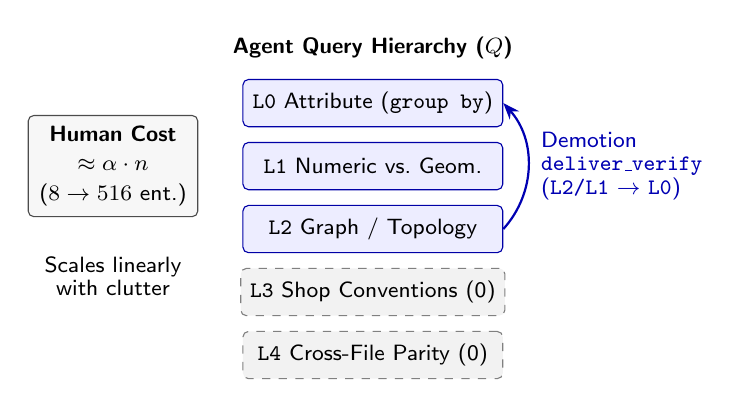
\begin{tikzpicture}[
  font=\sffamily\footnotesize,
  lvl/.style={draw=black!75, rounded corners=2pt, minimum width=33mm, minimum height=6.0mm, align=center, font=\sffamily\footnotesize},
  cov/.style={lvl, fill=blue!7, draw=blue!65!black},
  unc/.style={lvl, fill=black!5, draw=black!50, dashed},
  arr/.style={-{Stealth[length=2.1mm]}, thick, blue!70!black}
]
  \node[draw=black!70, fill=black!3, rounded corners=2pt, align=center, inner sep=4pt, font=\sffamily\footnotesize] (hum) at (-2.55, 0.85) {\textbf{Human Cost}\\[1pt]$\approx \alpha \cdot n$\\[1pt]($8 \to 516$ ent.)};
  \node[font=\sffamily\footnotesize, align=center] at (-2.55, -0.55) {Scales linearly\\[-1pt]with clutter};

  \node[cov] (l0) at (0.75, 1.65) {\texttt{L0} Attribute (\texttt{group by})};
  \node[cov] (l1) at (0.75, 0.85) {\texttt{L1} Numeric vs.\ Geom.};
  \node[cov] (l2) at (0.75, 0.05) {\texttt{L2} Graph / Topology};
  \node[unc] (l3) at (0.75, -0.75) {\texttt{L3} Shop Conventions (0)};
  \node[unc] (l4) at (0.75, -1.55) {\texttt{L4} Cross-File Parity (0)};

  \node[font=\sffamily\footnotesize\bfseries] at (0.75, 2.35) {Agent Query Hierarchy ($Q$)};
  \draw[arr] (l2.east) to[bend right=42] node[right, align=left, font=\sffamily\footnotesize, xshift=1pt] {Demotion\\[-1pt]\texttt{deliver\_verify}\\[-1pt](\texttt{L2/L1} $\to$ \texttt{L0})} (l0.east);
\end{tikzpicture}%
\label{fig:cost_asymmetry}
}%
\end{subfigure}%
\hfill
\begin{subfigure}[t]{0.50\textwidth}
\centering{
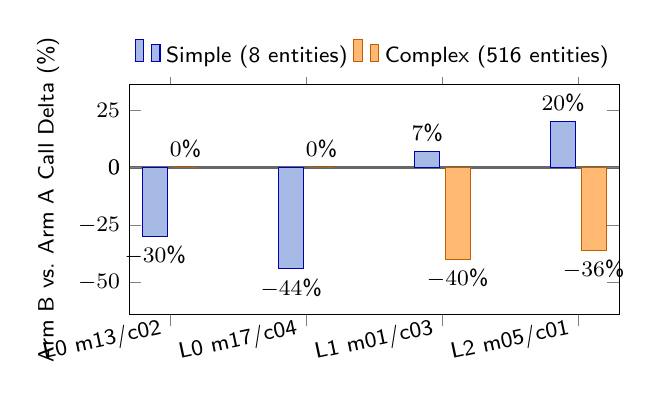
\begin{tikzpicture}
\begin{axis}[
  ybar,
  width=7.8cm, height=4.5cm,
  bar width=9pt,
  ymin=-64, ymax=36,
  ylabel={Arm B vs.\ Arm A Call Delta (\%)},
  label style={font=\sffamily\footnotesize},
  tick label style={font=\sffamily\footnotesize},
  symbolic x coords={L0 m13/c02, L0 m17/c04, L1 m01/c03, L2 m05/c01},
  xtick=data,
  x tick label style={font=\sffamily\footnotesize, rotate=12, anchor=east},
  ytick={-50,-25,0,25},
  extra y ticks={0},
  extra y tick style={grid=major, grid style={black!60, thick}},
  legend style={at={(0.5,1.03)}, anchor=south, legend columns=2, font=\sffamily\footnotesize, draw=none},
  nodes near coords={\pgfmathprintnumber{\pgfplotspointmeta}\%},
  nodes near coords align={vertical},
  nodes near coords style={font=\sffamily\footnotesize, text=black}
]
\addplot[fill=cyan!45!blue!35, draw=blue!70!black] coordinates {
  (L0 m13/c02, -30)
  (L0 m17/c04, -44)
  (L1 m01/c03, 7)
  (L2 m05/c01, 20)
};
\addplot[fill=orange!55!white, draw=orange!75!black] coordinates {
  (L0 m13/c02, 0)
  (L0 m17/c04, 0)
  (L1 m01/c03, -40)
  (L2 m05/c01, -36)
};
\legend{Simple (8 entities), Complex (516 entities)}
\end{axis}
\end{tikzpicture}%
\label{fig:scale_reversal}
}%
\end{subfigure}%
\caption{Cost asymmetry and scale-by-query-level interaction across 24 repair runs: (\emph{a}) asymmetric human ($\alpha \cdot n$) versus agent ($\beta + \gamma \cdot Q$) localization costs with \texttt{deliver\_verify} query-level demotion from \texttt{L2}/\texttt{L1} to \texttt{L0}; and (\emph{b}) Arm~B vs.\ Arm~A tool-call change ($\Delta\%$) across paired single-level tasks (\texttt{m13}/\texttt{c02}: \texttt{mut\_13}/\texttt{complex\_02}; \texttt{m17}/\texttt{c04}: \texttt{mut\_17}/\texttt{complex\_04}; \texttt{m01}/\texttt{c03}: \texttt{mut\_01}/\texttt{complex\_03}; \texttt{m05}/\texttt{c01}: \texttt{mut\_05}/\texttt{complex\_01}), illustrating \texttt{L0} fade-out versus the 56-percentage-point \texttt{L2} reversal\label{fig:query_and_reversal}}
\end{figure*}

\subsection{Scale-by-Query-Level Interaction Reversal}\label{sec:scale_level_reversal}

Disaggregating the 24 repair runs in \texttt{analyse\_levels.py} by Query Level $\times$ Entity Scale exposes an opposing structural interaction masked by aggregate pass rates (Fig.~\ref{fig:scale_reversal}; per-case table in Supplementary Material Table~S4, where \texttt{mut\_09\_sheet\_size} Arm~A and \texttt{mut\_19\_contour\_on\_zero} Arm~B lacked tool-call logs and are excluded from paired means):

\begin{enumerate}
\item \emph{Scale neutralizes {\upshape\texttt{L0}} attribute advantage}: On 8-entity drawings, structured hints cut tool calls by $-30\%$ (\texttt{mut\_13\_titleblock\_gone}: $10 \to 7$) and $-44\%$ (\texttt{mut\_17\_dim\_wrong\_layer}: $9 \to 5$). On 516-entity drawings, that gain vanishes to exact ties on both \texttt{complex\_02\_dim\_layer} ($5 \to 5$, $0\%$) and \texttt{complex\_04\_title\_blank} ($6 \to 6$, $0\%$). Because 43 of 45 dimensions sat cleanly on layer \emph{biaozhu} while 2 deviated, one \texttt{group by layer} script gave Arm~A free statistical contrast.
\item \emph{Scale triggers a 56-percentage-point {\upshape\texttt{L2}} reversal}: On single-polyline \texttt{mut\_05\_profile\_open}, reading \texttt{fix\_plan} added overhead ($5 \to 6$ calls, $+20\%$). Across 200 disconnected line segments concealing one 0.02~mm gap (\texttt{complex\_01\_profile\_open}), Arm~B saved $-36\%$ ($14 \to 9$), shifting by 56~percentage points: Arm~A calls surged $+180\%$ ($5 \to 14$) to write and debug graph traversal, while Arm~B calls rose only $+50\%$ ($6 \to 9$) by jumping directly to gap coordinates.
\end{enumerate}

Remaining paired cases match this mechanism: \texttt{L1} numeric \texttt{mut\_01\_bbox\_point} ($15 \to 16$, $+7\%$) flips on complex $+0.3\%$ override \texttt{complex\_03\_dim\_text} ($10 \to 6$, $-40\%$), while compound tasks \texttt{complex\_05\_two\_defects} ($11 \to 9$, $-18\%$) and \texttt{complex\_06\_all\_four} ($12 \to 10$, $-17\%$) yield blended savings. Pooling across scales at the level means (\texttt{L0}: $7.5 \to 5.8$ [$-23\%$], $n=4$; \texttt{L1}: $12.5 \to 11.0$ [$-12\%$], $n=2$; \texttt{L2}: $9.5 \to 7.5$ [$-21\%$], $n=2$) hides this divergence. Feedback value depends on whether scale lowers or raises agent self-discovery cost.

\subsection{Three Silent Failure Modes in Commercial CAD Automation and the Artifact Read-Back Axiom}\label{sec:cad_silent_failures}

While automating AutoCAD~2025 and SolidWorks~2025 via Windows COM for our cross-ecosystem suite, we documented three escalating silent failure modes mirroring checker-side skips:

\begin{enumerate}
\item \emph{Mode~1: Null returns without exceptions} (\texttt{None}/\texttt{False}): SolidWorks \texttt{CreateDrawView\allowbreak FromModelView3(part, "*Front", ...)} returns \texttt{None} on localized view strings (requiring \texttt{Create1st\allowbreak AngleViews2(model)}), and \texttt{ISheet.\allowbreak SetTemplateName} and \texttt{InsertTitle\allowbreak BlockTable} return \texttt{None} with zero file edits, leaving subsequent steps operating on empty objects unless return values are asserted.
\item \emph{Mode~2: Success flags with zero effect} (\texttt{True}): SolidWorks \texttt{IDrawingDoc.CreateLayer2} (7-arg) returns \texttt{True} and setting \texttt{IAnnotation.Layer = "biaozhu"} with \texttt{LayerOverride = 1} succeeds without error while exporting everything on layer~\texttt{0}; similarly, on \texttt{part-006}, \texttt{InsertModelAnnotations3} (6-arg) succeeded while emitting 0 dimensions.
\item \emph{Mode~3: Void return with command buffer truncated.} AutoCAD~2025 \texttt{SendCommand} executing multi-entity LISP \texttt{(progn (entmake ...))} block definitions truncated mid-buffer, leaving \texttt{BLOCKS: []} and orphan \texttt{ATTDEF}s until trimmed to a 3-\texttt{ATTDEF} \texttt{GB-TITLE} block with \texttt{(cons 66 1)}.
\end{enumerate}

All three modes establish a shared engineering rule, the artifact read-back axiom: \textbf{when driving external CAD kernels, ``API call returned cleanly'' and ``intended artifact materialized'' are independent events; only independent symbolic parsing of the persisted disk file separates them.} Where Windows COM type libraries failed (\texttt{EnsureDispatch} and \texttt{makepy} errored), we resolved exact call bindings via direct \texttt{.NET} interop reflection over \texttt{SolidWorks.Interop.swconst.dll} (extracting all 818 \texttt{swUserPreferenceToggle\_e} constants, 6-arg \texttt{InsertModelAnnotations3}, 7-arg \texttt{CreateLayer2}, and \texttt{swUnitsLinear = 47}) alongside AutoCAD \texttt{VARIANT} and backoff wrappers; full harness details appear in Supplementary Material (Section~S4).

\subsection{Protocol Discipline, Cross-Format Depth, and Design-Intent Non-Goals}\label{sec:protocol_boundaries}

Three hard operational boundaries bound how \texttt{cad-deliver-mcp} should be deployed:

\begin{enumerate}
\item \emph{Protocol discipline, not a security sandbox.} As implemented in \texttt{src/cad\_deliver/state\_machine.py}, \texttt{StagingStore} detects post-verification tampering via SHA-256 checks (\texttt{E\_HASH\_CHANGED}). An agent with workspace write access can still modify files and open a new \texttt{deliver\_stage} record; 2PC guarantees auditable visibility (\texttt{attempts}, UTC \texttt{history}, and digests in \texttt{deliver://audit/\{staging\_id\}}) instead of sandbox confinement.
\item \emph{Format-stratified verification depth.} Full entity, layer, attribute, dimension, and closure checks apply strictly to DXF (Table~\ref{tab:format_capabilities}). STEP validates text schemas and raw bounding boxes without a 3D B-rep kernel; PDF checks pages, ISO~216 bounds, and vector text; and \texttt{.sldprt}/\texttt{.sldasm} binaries verify existence, byte size, and binary signatures only.
\item \emph{Design intent and manufacturability remain out of scope.} Checking covers drafting-standard expression, not whether fits (\texttt{H7/g6}), materials, tolerance stacks, or manufacturability are sound. Under \texttt{cli.py --profile half}, \texttt{delivery.json} writes three explicit exclusions into \texttt{not\_checked} confirming that \texttt{PASS} certifies readiness for engineering sign-off without replacing it.
\end{enumerate}

%%%%%%%%%%%%%%%%%%%%%%%%%%%%%%%%%%%%%%%%%%%%%%%%%%%%%%%%%%%%%%%%%%%%%%%%%%%%%%%
\section{Conclusion and Threats to Validity}\label{sec:conclusion}

\subsection{Conclusion}\label{sec:concl_summary}

This paper operationalizes the pre-delivery verification principle \emph{abstention is not a pass}: \texttt{PASS} holds only when every required dimension executed, preconditions held, and no blocking violation occurred; unexamined states surface explicitly as \texttt{UNKNOWN} (exit code~\texttt{2}). Built on 4,682~LOC and passing all 74~automated tests, \texttt{cad-deliver-mcp} isolates \texttt{parsers/} from pure-function \texttt{geometry/} and \texttt{rules/} through a live-object-free \texttt{ParsedDrawing} contract and static import checks, pairs a seven-role drafting layer ontology with six calibrated rules across separated rule, profile, and severity tables, and enforces SHA-256 two-phase commit delivery via MCP.

On our 50-drawing benchmark, \texttt{G3} achieves 20/20 (100.0\%) exact-code recall (95\% Clopper--Pearson lower bound 86.1\%) and 0/30 (0.0\%) compliant false positives (upper bound 9.5\%) at 12.37~ms median latency ($p_{95}=50.75$~ms; 2.07~ms net rule overhead), with five rules each contributing $-4$ unique detections under LOO ablation and \texttt{gb.dim\_text} calibrated on native scaling cases. Static-syntax scripts (\texttt{G2.5}, \texttt{LEGACY\_COMPAT}) and AutoCAD \texttt{.dws} detect 0/20 defects (Section~\ref{sec:eval}), while \texttt{qwen3-vl-plus} exhibits a visual/geometric (11/12) versus layer/sheet metadata (0/8) cliff alongside 17/30 compliant false positives. Across 15 identical parts, native AutoCAD~2025 exports yield 15/15 \texttt{PASS} versus 0~\texttt{PASS} / 2~\texttt{FAIL} / 13~\texttt{UNKNOWN} on SolidWorks~2025 exports, backed by an exhaustive audit of 129 registry entries and 818 user-preference constants. Finally, our mutation-purity criterion, \texttt{L0}--\texttt{L4} query taxonomy (revealing a 56-percentage-point reversal on 516-entity \texttt{L2} repair tasks), and ratio-dispersion criterion provide domain-independent tools for CAD agent evaluation.

\subsection{Internal and Construct Threats to Validity}\label{sec:internal_threats}

Three internal and construct threats bound our claims:

\begin{enumerate}
\item \emph{Absence of human expert evaluation.} This study did not execute human expert review experiments or measure engineer review-hour savings in production. Rule thresholds derive from GB/T standards, so our 0/30 false-positive result (95\% UB 9.5\%) reflects formal conformance instead of subjective shop-floor approval, and automated baselines (\texttt{.dws} and \texttt{qwen3-vl-plus}) do not substitute for human-subject evidence. A blinded 32-task protocol (\texttt{CASE-01}--\texttt{CASE-32}: 4 practice + 28 scored comprising 18 defective and 10 compliant drawings) and script (\texttt{scripts/analyze\_human\_eval.py}) are archived in \texttt{benchmarks/human\_eval/PROTOCOL.md} and can be executed as-is.
\item \emph{Rendering pipeline trade-off} (\texttt{TextPolicy.IGNORE}): Suppressing \texttt{ezdxf} SHX rendering avoided CJK tofu blocks and label shifts yet hid internal \texttt{DIMENSION} measurement strings (Section~\ref{sec:render_debug}), leaving \texttt{dims\_ok} unanswerable and inflating compliant FPs (17/30). Cleanly displaying dimension numerals would lower FP rates without closing the 11/12 visual versus 0/8 symbolic metadata cliff.
\item \emph{Synthetic defect and query-level coverage gaps.} Our 20 synthetic mutations omit overridden dimension text (leaving \texttt{gb.dim\_text} at 0 LOO drop despite activation on \texttt{part-012}/\texttt{013} and \texttt{complex\_03}/\texttt{06}), and all 24 repair runs span \texttt{L0}--\texttt{L2} (\texttt{L3 = 0, L4 = 0}) without restricting control-arm read access.
\end{enumerate}

\subsection{External Threats to Validity, Ecosystem Boundaries, and Future Work}\label{sec:external_threats}

External generalizability is bounded by sample size ($n=50$ yields 95\% binomial intervals $[86.1\%, 100\%]$ recall and $[0\%, 9.5\%]$ FP; subclasses $n \le 4$ yield 47.3\% lower bound and remain mechanistic), cross-ecosystem exporter structure (AutoCAD~2025 yields 15/15 \texttt{PASS}, whereas weak-layer SolidWorks~2025 yields 13/15 \texttt{UNKNOWN} until enterprise templates embed layers and sheet formats), and format granularity (Table~\ref{tab:format_capabilities}).

Four directions anchor future work: (1) adding overridden dimension-text mutations alongside \texttt{L3} workshop-convention twins and \texttt{L4} 2D-DXF/3D-STEP consistency benchmarks under restricted baseline file access (Section~\ref{sec:query_taxonomy}); (2) adding native ASME~Y14.5/Y14.1 and ISO~128/13567 profiles plus lightweight B-rep backends for STEP; (3) embedding standardized layers, sheet formats, and attributed blocks inside SolidWorks \texttt{.drwdot} templates; and (4) executing the \texttt{benchmarks/human\_eval/} study across at least 3 practicing mechanical engineers split across \texttt{cad} and \texttt{png} conditions (measuring recall, FP, Fleiss' $\kappa$, and review latency).

%%%%%%%%%%%%%%%%%%%%%%%%%%%%%%%%%%%%%%%%%%%%%%%%%%%%%%%%%%%%%%%%%%%%%%%%%%%%%%%
\vspace{-4pt}
\bibliographystyle{asmejour}
\setlength\bibsep{-1.8pt}
\bibliography{references}

\end{document}
